\documentclass[12pt, a4paper]{article}
\usepackage{graphicx}
\usepackage[T1]{fontenc}
\usepackage[utf8]{vietnam}
\usepackage{geometry}
\usepackage{caption}
\usepackage{float}
\usepackage{ulem}
\usepackage{changepage}
\usepackage{tocloft}
\usepackage{ragged2e}
\usepackage{array}
\usepackage{tcolorbox}
\usepackage{titlesec}
\usepackage{enumitem}
% Cấu hình cho \section
\titleformat{\section}
{\normalfont\fontsize{20}{18}\bfseries}{\thesection}{1em}{}
% Cấu hình cho \subsection
\titleformat{\subsection}
{\normalfont\fontsize{17}{18}\bfseries}{\thesubsection}{1em}{}
% Cấu hình cho \subsubsection
\titleformat{\subsubsection}
{\normalfont\fontsize{15}{18}\bfseries}{\thesubsubsection}{1em}{}
\usepackage{setspace}
\geometry{
	a4paper,
	left=2.5cm,
	right=2cm,
	top=2.5cm,
	bottom=3cm,
}
% Thiết lập các mục lục và danh sách
\renewcommand{\contentsname}{\fontsize{20}{24}\bfseries\MakeUppercase{Mục Lục}}
\renewcommand{\listtablename}{\fontsize{20}{24}\bfseries\MakeUppercase{Danh Sách Bảng}}
\renewcommand{\listfigurename}{\fontsize{20}{24}\bfseries\MakeUppercase{Danh Sách Hình Ảnh}}

\begin{document}
	\begin{center} 
		\setstretch{1.5}
		\large TỔNG LIÊN ĐOÀN LAO ĐỘNG VIỆT NAM 
		\\ \textbf{TRƯỜNG ĐẠI HỌC TÔN ĐỨC THẮNG} 
		\\ \textbf{KHOA CÔNG NGHỆ THÔNG TIN} 
		\large
		\begin{figure}[H]
			\centering
			
\includegraphics[width=0.2\textwidth]{logo_tdtu.jpg}
			\label{fig:logoTDT_1}
		\end{figure}
		{\large \textbf{ĐỒ ÁN CUỐI KỲ\\}}
		{\large \textbf{MÔN GIAO THỨC VÀ MẠNG MÁY TÍNH}}
		\\ [35pt]
		{\huge \textbf{THIẾT KẾ VÀ TRIỂN KHAI HỆ THỐNG MẠNG MÁY TÍNH CHO TRƯỜNG ĐẠI HỌC SÀI GÒN CÓ 3 CHI NHÁNH Ở TPHCM}}\\ [35pt]
		\begin{flushright}
			{\large \textit{Giảng viên hướng dẫn: }} 
			\textbf{ThS. TRƯƠNG ĐÌNH TÚ } \\
			{\large \textit{Người thực hiện: }} 
			\textbf{NGUYỄN AN - 52100950} \\
			\textbf{ĐINH PHƯƠNG MY  - 52100703} \\
			\textbf{NGUYỄN HÀO NAM - 52100979} \\	
			{\large \textit{Lớp: }} 
			\textbf{21050401 } \\
			{\large \textit{Khóa: }} 
			\textbf{25} \\ [35pt]
		\end{flushright} 
		{\large \textbf{THÀNH PHỐ HỒ CHÍ MINH, NĂM 2024}}\\
	\end{center}
	
	\newpage
	\begin{center} 
		\setstretch{1.5}
		\large TỔNG LIÊN ĐOÀN LAO ĐỘNG VIỆT NAM 
		\\ \textbf{TRƯỜNG ĐẠI HỌC TÔN ĐỨC THẮNG} 
		\\ \textbf{KHOA CÔNG NGHỆ THÔNG TIN} 
		\large
		\begin{figure}[H]
			\centering
			
\includegraphics[width=0.2\textwidth]{logo_tdtu.jpg}
			\label{fig:logoTDT_1}
		\end{figure}
		{\large \textbf{ĐỒ ÁN CUỐI KỲ\\}}
		{\large \textbf{MÔN GIAO THỨC VÀ MẠNG MÁY TÍNH}}
		\\ [35pt]
		{\huge \textbf{THIẾT KẾ VÀ TRIỂN KHAI HỆ THỐNG MẠNG MÁY TÍNH CHO TRƯỜNG ĐẠI HỌC SÀI GÒN CÓ 3 CHI NHÁNH Ở TPHCM}}\\ [35pt]
		\begin{flushright}
			{\large \textit{Giảng viên hướng dẫn: }} 
			\textbf{ThS. TRƯƠNG ĐÌNH TÚ } \\
			{\large \textit{Người thực hiện: }} 
			\textbf{NGUYỄN AN - 52100950} \\
			\textbf{ĐINH PHƯƠNG MY  - 52100703} \\
			\textbf{NGUYỄN HÀO NAM - 52100979} \\	
			{\large \textit{Lớp: }} 
			\textbf{21050401 } \\
			{\large \textit{Khóa: }} 
			\textbf{25} \\ [35pt]
		\end{flushright} 
		{\large \textbf{THÀNH PHỐ HỒ CHÍ MINH, NĂM 2024}}\\
	\end{center}
	
	\newpage
	\begin{center}
		\textbf{\Large LỜI CÁM ƠN}\\ [15pt]
	\end{center}
	\par
	\large
	\setstretch{1.5}
	\hspace{0.75cm}Lời đầu tiên, nhóm 15 xin gửi lời cám ơn chân thành đến ThS. Trương Đình Tú. Trong quá trình học tập và tìm hiểu môn học Giao Thức Và Mạng Máy Tính, nhóm 15 đã nhận được sự quan tâm, giúp đỡ, hướng dẫn rất tận tình, tâm huyết của thầy. Thầy đã giúp nhóm 15 tích lũy thêm nhiều kiến thức để có cái nhìn sâu sắc và định hướng hoàn thiện hơn trong cuộc sống. Từ những kiến thức mà thầy truyền tải, nhóm 15 đã dần trả lời được những câu hỏi khó trong bộ môn, cũng như hiểu và giải được những bài tập mà thầy giao. Thông qua bài báo cáo cuối kỳ này, nhóm 15 xin trình bày lại những gì mà mình đã tìm hiểu về môn học Giao Thức Và Mạng Máy Tính gửi đến thầy. \par
	\hspace{0.75cm}Có lẽ kiến thức là vô hạn mà sự tiếp nhận kiến thức của bản thân mỗi người luôn luôn tồn tại những hạn chế nhất định. Do đó, trong quá trình hoàn thành bài báo cáo cuối kỳ này, chắc chắn nhóm 15 sẽ không tránh khỏi những thiếu sót. Bản thân nhóm 15 rất mong nhận được những góp ý đến từ thầy để bài báo cáo cuối kỳ của nhóm 15 được hoàn thiện hơn.\par
	\hspace{0.75cm}Kính chúc thầy có nhiều sức khỏe, hạnh phúc và thành công trên con đường giảng dạy của mình để có thể dìu dắt nhiều thế hệ sinh viên trong tương lai.\par

	\newpage
	\begin{center}
		\textbf{\Large ĐỒ ÁN ĐƯỢC HOÀN THÀNH\\TẠI TRƯỜNG ĐẠI HỌC TÔN ĐỨC THẮNG}\\ [15pt]
	\end{center}
	\par 
	\large 
	\setstretch{1.5}
	\hspace{0.75cm}Nhóm 15 xin cam đoan đây là sản phẩm đồ án của riêng nhóm và được sự hướng dẫn của ThS. Trương Đình Tú. Các nội dung nghiên cứu, kết quả trong đề tài này là trung thực và chưa công bố dưới bất kỳ hình thức nào trước đây. Những số liệu trong các bảng biểu phục vụ cho việc phân tích, nhận xét, đánh giá được chính tác giả thu thập từ các nguồn khác nhau có ghi rõ trong phần tài liệu tham khảo.\par
	\hspace{0.75cm}Ngoài ra, trong đồ án còn sử dụng một số nhận xét, đánh giá cũng như số liệu của các tác giả khác, cơ quan tổ chức khác đều có trích dẫn và chú thích nguồn gốc.\par
	\hspace{0.75cm}Nếu phát hiện có bất kỳ sự gian lận nào chúng em xin hoàn toàn chịu trách nhiệm về nội dung đồ án của mình. Trường đại học Tôn Đức Thắng không liên quan đến những vi phạm tác quyền, bản quyền do chúng em gây ra trong quá trình thực hiện (nếu có).
	\begin{flushright}
		{\large \textit{TP. Hồ Chí Minh, ngày 10 tháng 05  năm 2024}} \\		
		\begin{adjustwidth}{9cm}{1cm}
			\begin{center}		
				{\large {Tác giả\\
						(ký tên và ghi rõ họ tên)\\
						Nguyễn An\\
						Đinh Phương My\\
						Nguyễn Hào Nam \\
				}} 
			\end{center}
		\end{adjustwidth}
	\end{flushright}					
	
	\newpage
	\begin{center}
		{\Large \textbf{TÓM TẮT}}\\ [15pt]
	\end{center}
	\par
	\large
	\setstretch{1.5} 
	\hspace{0.75cm}Ngày nay, để thiết kế một mô hình mạng máy tính hiệu quả và dễ vận hành là yếu tố quan trọng đối với việc đáp ứng nhu cầu công việc và hoạt động của các công ty, tổ chức, cũng như đời sống cá nhân. Trong đồ án này, nhóm 15 sẽ tìm hiểu, phân tích và thiết kế mô hình mạng máy tính cho trường Đại học Sài gòn với 3 chi nhánh tại Thành phố Hồ Chí Minh, đồ án được chia thành các phần sau:\par
	\hspace{0.75cm}Chương 1: Giới thiệu và khảo sát đề tài\par
	\hspace{0.75cm}Trong phần này, nhóm 15 sẽ giới thiệu về đề tài của đồ án và khảo sát các yêu cầu và nhu cầu của trường Đại học Sài Gòn, cũng như đưa ra lý do cần thiết phải thiết kế một mô hình mạng máy tính mới. Nhóm 15 sẽ nêu ra các mục tiêu và lợi ích mà mô hình mạng mới đem lại cho trường Đại học Sài Gòn.\par
	\hspace{0.75cm}Chương 2: Mô hình hệ thống\par
	\hspace{0.75cm}Trong phần này, nhóm 15 sẽ thiết kế topology mạng sử dụng phần mềm mô phỏng Cisco Packet Tracer. Mô hình mạng sẽ được thiết kế theo mô hình 3 tầng gồm Access Layer, Distribution Layer và Core Layer. Em sẽ áp dụng các kiến thức đã học như cấu hình chia VLAN, inter-VLAN, STP, EtherChannel, DHCPv4, DHCPv6, Routing để triển khai mô hình mạng. Nhóm 15 cũng sẽ sử dụng kỹ thuật chia subnet, VLSM để chia các subnet cho hệ thống mạng sao cho tiết kiệm địa chỉ IP nhất. Cấu hình song song IPv4 và IPv6 cũng sẽ được thực hiện.\par
	\hspace{0.75cm}Ngoài ra, nhóm 15 cũng sẽ thiết kế mạng có tính dự phòng bằng cách sử dụng STP, EtherChannel để đảm bảo tính khả dụng và tin cậy của mạng. Nhóm 15 cũng sẽ triển khai cấu hình định tuyến động (DYNAMIC ROUTING) sử dụng OSPF hoặc EIGRP để tối ưu hóa quản lý định tuyến trong mạng. \par
	\hspace{0.75cm}Chương 3: Triển khai dịch vụ mạng 	
	\par
	\hspace{0.75cm}Trong phần này, nhóm 15 sẽ cài đặt và cấu hình đầy đủ các dịch vụ mạng như DHCP Server, DNS Server, Web Server, FTP server, Mail server trong hệ thống mạng. Nhóm 15 sẽ tạo một trang web đơn giản bằng HTML trên Web server và đảm bảo các clients trong mạng có thể kết nối đến các Domain name và Web server đã tạo. Nhóm 15 cũng sẽ tạo một tên domain trên Mail Server và tạo các user để gửi Email qua lại với nhau. Ngoài ra, nhóm 15 cũng sẽ triển khai phủ sóng wifi tại các nơi cần thiết trong trường Đại học Sài Gòn.\par
	\hspace{0.75cm}Chương 4: Cấu hình bảo mật\par
	\hspace{0.75cm}Trong phần này, nhóm 15 sẽ triển khai các cấu hình bảo mật để đảm bảo tính an toàn và bảo mật cho hệ thống mạng. Các biện pháp bảo mật sẽ được áp dụng như Firewall, ACL, VPN, AAA (Authentication, Authorization, Accounting), 802.1X, đảm bảo tính bảo mật cho các dịch vụ mạng đã triển khai trong phần trước như DHCP, DNS, Web, FTP, Mail. Ngoài ra, nhóm 15 cũng sẽ triển khai các biện pháp bảo mật cho mạng không dây (Wifi) như sử dụng mã hóa WPA2, Radius Server, giới hạn phạm vi sóng Wifi, đảm bảo tính riêng tư và an toàn cho người dùng.\par
	\hspace{0.75cm}Chương 5: Kiểm thử và đánh giá\par
	\hspace{0.75cm}Trong phần này, nhóm 15 sẽ tiến hành kiểm thử, đánh giá hệ thống mạng đã triển khai. Nhóm 15 sẽ kiểm tra tính ổn định, tính khả dụng, tính an toàn của hệ thống mạng bằng cách kiểm tra kết nối, đồng bộ hoá, đồng bộ hóa định tuyến, kiểm tra các dịch vụ mạng đã triển khai. Ngoài ra, nhóm 15 cũng sẽ đánh giá hiệu năng và độ tin cậy của hệ thống mạng dựa trên các tiêu chí đã đề ra trong phần giới thiệu và khảo sát đề tài.\par
	\hspace{0.75cm}Chương 6: Tổng kết và đề xuất\par
	\hspace{0.75cm}Trong phần này, nhóm 15 sẽ tổng kết lại các kết quả đạt được trong đồ án, đưa ra nhận xét và đánh giá tổng thể về mô hình mạng đã triển khai. Nếu có, nhóm 15 sẽ đưa ra những đề xuất, gợi ý để cải thiện hoặc mở rộng mô hình mạng trong tương lai. Cuối cùng, nhóm 15 sẽ kết luận và đưa ra những kết luận cuối cùng về đề tài và những đóng góp của đồ án đối với trường Đại học Sài Gòn. \par
	\newpage
	
	\begin{center}
		\setstretch{1.5}
		\tableofcontents
	\end{center}
	
	\newpage
	% Danh mục bảng biểu
	\setstretch{1.5}
	\listoftables
	
	% Danh mục hình ảnh
	\setstretch{1.5}
	\listoffigures
	
	\newpage
	\section{GIỚI THIỆU VÀ KHẢO SÁT}
	\subsection{Giới thiệu đề tài}
	\begin{flushleft}
		\setstretch{1.5}
		\hspace{1.5cm}Đề tài "Thiết kế và triển khai hệ thống mạng máy tính cho trường đại học Sài Gòn có 3 chi nhánh ở thành phố Hồ Chí Minh" là một đề tài có tính ứng dụng cao trong thực tế, giúp nâng cao chất lượng giáo dục và quản lý của nhà trường. \\
		\hspace{1.5cm}Trong đề tài này, chúng ta sẽ thiết kế và triển khai một hệ thống mạng máy tính đáp ứng được các yêu cầu của trường đại học Sài Gòn và các chi nhánh của nó ở thành phố Hồ Chí Minh, đảm bảo hiệu quả sử dụng và an toàn thông tin.
		\\\hspace{1.5cm}Các yêu cầu của hệ thống mạng máy tính bao gồm: 
		\begin{itemize}[leftmargin=2.3cm, itemsep=0pt, topsep=0pt]
			\item Tốc độ truy cập nhanh.
			\item Độ tin cậy cao.
			\item Bảo mật thông tin.
			\item Khả năng mở rộng.
			\item Tính linh hoạt.
			\item Dễ quản lý. 
		\end{itemize}
		\hspace{1.5cm}Hệ thống mạng máy tính cần phải được thiết kế để đáp ứng được nhu cầu sử dụng của sinh viên và giảng viên, cũng như các bộ phận quản lý và hỗ trợ kỹ thuật. Hệ thống phải đảm bảo hiệu suất cao, bảo mật tối ưu, và khả năng phục vụ số lượng lớn người dùng đồng thời.
		\\\hspace{1.5cm}Để thực hiện đề tài này, nhóm 15 sẽ thực hiện các công việc như sau:
		\begin{itemize}[leftmargin=2.3cm, itemsep=0pt, topsep=0pt]
			\item  Đánh giá nhu cầu sử dụng của trường đại học Sài Gòn và các chi nhánh của nó ở thành phố Hồ Chí Minh, bao gồm số lượng người dùng, yêu cầu về băng thông, và các ứng dụng sử dụng trong học tập và quản lý.
			\item  Thiết kế kiến trúc hệ thống mạng máy tính gồm các thành phần như router, switch, server, và các thiết bị mạng không dây khác, đảm bảo tính hợp lý và hiệu quả.
			\item  Lựa chọn các thiết bị mạng phù hợp với yêu cầu của hệ thống, đảm bảo tính tương thích và khả năng mở rộng trong tương lai, đồng thời xem xét các yếu tố về chi phí và hiệu suất.
			\item  Cài đặt và cấu hình các thiết bị mạng theo mô hình đã thiết kế, bao gồm việc triển khai các biện pháp bảo mật như tường lửa, VPN, và hệ thống giám sát an ninh mạng.
			\item  Kiểm tra và đánh giá hiệu suất của hệ thống mạng máy tính thông qua các bài kiểm tra thực tế, đánh giá độ tin cậy và tốc độ truy cập, đảm bảo hệ thống hoạt động ổn định.
			\item  Đưa ra các giải pháp nâng cấp và mở rộng hệ thống mạng máy tính trong tương lai, bao gồm các kế hoạch dự phòng, bảo trì định kỳ, và cập nhật công nghệ mới.
		\end{itemize}
		\hspace{1.5cm}Kết quả của đề tài này sẽ giúp trường đại học Sài Gòn và các chi nhánh của nó ở thành phố Hồ Chí Minh có một hệ thống mạng máy tính tốt, đáp ứng được nhu cầu sử dụng hiện tại và tương lai. Hệ thống sẽ góp phần nâng cao hiệu suất làm việc, tối ưu hóa chi phí đầu tư, và tạo nền tảng vững chắc cho sự phát triển của nhà trường trong thời đại công nghệ số.
	\end{flushleft}
	
	\newpage
	\subsection{Mô tả đề tài}
	\begin{flushleft}
		\setstretch{1.5}
		\hspace{1.5cm}Triển khai thiết kế hệ thống mạng cho trường đại học Sài Gòn với các dịch vụ cho server là một công việc quan trọng trong quá trình xây dựng hệ thống mạng máy tính.
		\\\hspace{1.5cm}Dưới đây là mô tả về một số dịch vụ cơ bản và mục đích của từng dịch vụ đó:
		\begin{itemize}[leftmargin=0.75cm, itemsep=0pt, topsep=0pt]
			\setstretch{1.5}\item Dịch vụ web: Dịch vụ này cho phép các người dùng truy cập vào các trang web của trường. Mục đích chính là cung cấp thông tin về trường, các khoá học, các hoạt động và tin tức của trường cho người dùng.
			\item  Dịch vụ email: Dịch vụ này cho phép người dùng gửi và nhận email trên hệ thống của trường. Mục đích chính là giúp người dùng giao tiếp và trao đổi thông tin với nhau một cách nhanh chóng và tiện lợi.
			\item  Dịch vụ lưu trữ tập tin: Dịch vụ này cho phép người dùng lưu trữ và truy cập các tập tin trên server của trường. Mục đích chính là cung cấp cho người dùng một nơi để lưu trữ và chia sẻ các tài liệu, bài giảng, nội dung học tập và công việc của mình.
			\item Dịch vụ FTP: Dịch vụ này cho phép người dùng tải lên và tải xuống các tập tin trên server của trường. Mục đích chính là hỗ trợ việc trao đổi và chia sẻ các tập tin lớn giữa các người dùng.
			\item Dịch vụ đăng nhập từ xa: Dịch vụ này cho phép người dùng truy cập vào hệ thống từ xa bằng cách sử dụng một ứng dụng đăng nhập từ xa. Mục đích chính là cung cấp cho người dùng khả năng truy cập vào hệ thống từ bất kỳ đâu và bất kỳ thiết bị nào có kết nối internet.
		\end{itemize}
	\end{flushleft}
	
	\newpage
	\subsection{Khảo sát thực tế}
	\begin{flushleft}
		\setstretch{1.5}
		\hspace{1.5cm} Qua việc khảo sát trụ tại trụ sở chính và các chi nhánh, nhóm 15 thu thập được các thông tin sau:
		\begin{itemize}[leftmargin=1.7cm, itemsep=0pt, topsep=0pt]
			\item Tòa A 
			\begin{itemize}[leftmargin=1cm, itemsep=0pt, topsep=0pt]
				\item Phòng Server: Chứa các máy chue của dịch vụ triển khai như DNS, Web, Email.\\
				\item Phòng Đào tạo: Nơi cung cấp các khóa học, chương trình đào tạo, và các hoạt động liên quan đến giáo dục và đào tạo. Các khóa học có thể bao gồm các khóa học cơ bản và nâng cao, chương trình đào tạo cho giáo viên, hoặc các khóa đào tạo chuyên môn cho các chuyên gia trong các lĩnh vực khác nhau. Phòng đào tạo cũng có thể giúp đỡ các sinh viên trong việc lựa chọn chương trình đào tạo phù hợp với nhu cầu của họ và hướng dẫn các sinh viên trong các hoạt động nghiên cứu khoa học. \
			\end{itemize}
			\item Tòa B:
			\begin{itemize}[leftmargin=1cm, itemsep=0pt, topsep=0pt]
				\item Phòng Công tác sinh viên: Nơi giúp đỡ và hỗ trợ cho sinh viên trong các hoạt động ngoại khóa, tư vấn học tập, hướng dẫn tìm việc làm, hỗ trợ tài chính và các hoạt động xã hội. Nó cũng cung cấp thông tin và hướng dẫn cho các sinh viên về các chính sách và quy định của trường học hoặc tổ chức giáo dục. \\
				\item Phòng Hành chính: Nơi quản lý các hoạt động hành chính và hỗ trợ cho các bộ phận khác trong trường học hoặc tổ chức giáo dục. Các công việc hành chính bao gồm quản lý văn bản, lưu trữ tài liệu, quản lý hồ sơ, quản lý dữ liệu, và hỗ trợ các bộ phận khác trong trường học hoặc tổ chức giáo dục. \
			\end{itemize}
			\item Tòa C: Gồm những phòng máy dùng để phục vụ cho việc học và thực hành trên máy tính.
			\item Tòa D:
			\begin{itemize}[leftmargin=1cm, itemsep=0pt, topsep=0pt]
				\item Hội trường: Một không gian lớn được sử dụng cho các sự kiện, buổi hội thảo, hội nghị, lễ kỷ niệm, v.v. Hội trường thường được trang bị đầy đủ các thiết bị âm thanh, ánh sáng và đa phương tiện để hỗ trợ các hoạt động trình diễn, thuyết trình và biểu diễn. Một số hội trường cũng có thể được trang bị các thiết bị quay phim, ghi âm và truyền hình để thuận tiện cho việc ghi lại các sự kiện hoặc phát sóng trực tuyến.\\
				\item Thư viện: Khu vực chứa và cung cấp tài liệu học liệu và nghiên cứu đa dạng cho cả sinh viên và giảng viên. Thư viện cung cấp không chỉ sách và tài liệu in mà còn tài nguyên điện tử, cơ sở dữ liệu trực tuyến, và các công cụ nghiên cứu khác. Nó cũng là nơi cung cấp dịch vụ mượn sách, hỗ trợ tìm kiếm thông tin, và cung cấp không gian làm việc yên tĩnh và thuận tiện cho học và nghiên cứu. \
			\end{itemize}
		\end{itemize}
	\end{flushleft}
	
	\newpage
	\section{MÔ HÌNH HỆ THỐNG}
	\subsection{Sơ đồ luận lý (Logical Topology)}
	\begin{figure}[H]
		\centering
		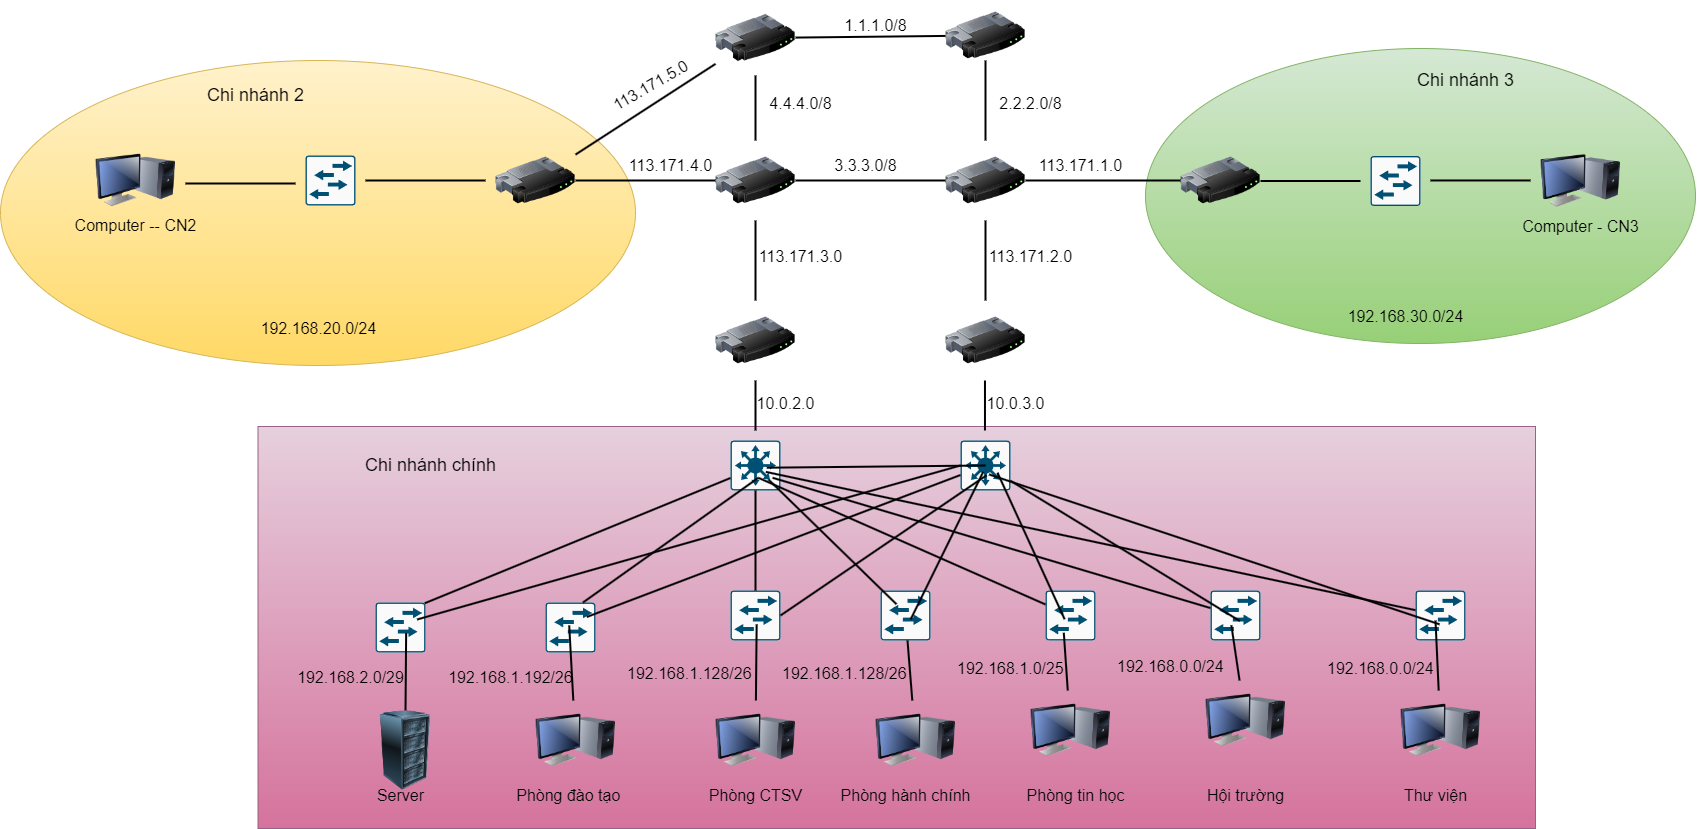
\includegraphics[width=0.95\textwidth]{sodolyluan.png}
		\caption{Sơ đồ luận lý} 
	\end{figure}
	\subsection{Sơ đồ vật lý (Physical Topology)}
	\begin{figure}[H]
		\centering
		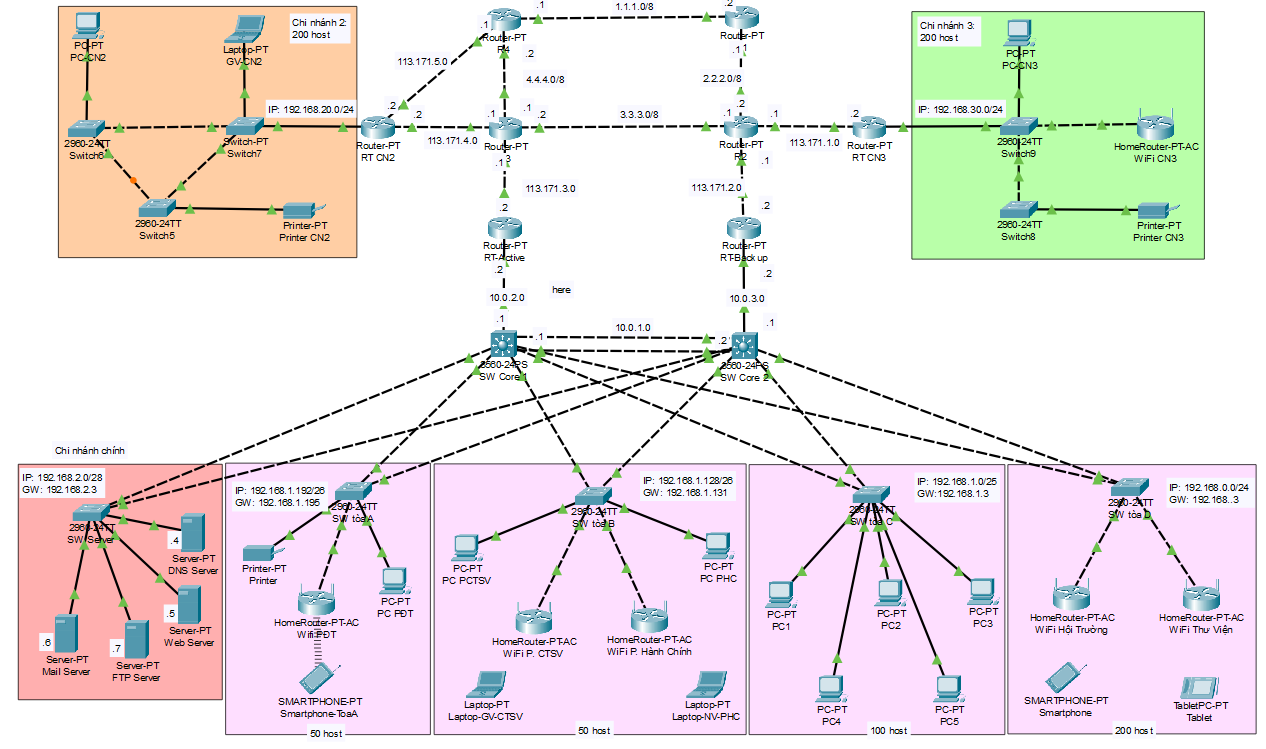
\includegraphics[width=0.95\textwidth]{sodovatly.png}
		\caption{Sơ đồ vật lý} 
	\end{figure}
	\newpage
	\section{THÔNG TIN CÀI ĐẶT CẤU HÌNH HỆ THỐNG}
	\subsection{Thông tin vlan, interface vlan trong hệ thống} 
	\subsubsection{\textit{Thông tin vlan}}
	\begin{table}[h]
		\centering
		\caption{Bảng thông tin các vlan}
		\begin{tabular}{|c|c|c|c|c|}
			\hline
			\textbf{Tên Vlan} & \textbf{Vlan ID} & \textbf{Port} & \textbf{Số lượng} & \textbf{Mô tả} \\
			\hline
			Vlan-Toa-D & 14 & Fa0/1- & 200 & \\
			\hline
			Vlan-Toa-C & 13 & Fa0/1- & 100 & \\
			\hline
			Vlan-Toa-B & 12 & Fa0/1- & 50 & \\
			\hline
			Vlan-Toa-A & 11 & Fa0/1- & 50 & \\
			\hline
			Vlan-Server & 10 & Fa0/10-13 & 4 & \\
			\hline
		\end{tabular}
	\end{table}
	\subsubsection{\textit{Thông tin interface vlan}}
	
	\begin{table}[h]
		\centering
		\caption{Bảng thông tin các interface vlan}
		\begin{tabular}{|c|c|c|c|c|}
			\hline
			\textbf{Thiết bị} & \textbf{Interface} & \textbf{IP Address/Prefix} & \textbf{Default Gateway} & \textbf{Broadcast} \\
			\hline
			SW-CORE-1 & Vlan 10 & 192.168.2.1/28 & 192.168.2.3 & 192.168.2.14\\
			\hline
			SW-CORE-1 & Vlan 11 & 192.168.1.193/26 & 192.168.1.195 & 192.168.1.255\\
			\hline
			SW-CORE-1 & Vlan 12 & 192.168.1.129/26 & 192.168.1.131 & 192.168.1.192\\
			\hline
			SW-CORE-1 & Vlan 13 & 192.168.1.1/25 & 192.168.1.3 & 192.168.1.128\\
			\hline
			SW-CORE-1 & Vlan 14 & 192.168.0.1/24 & 192.168.0.3 & 192.168.0.255\\
			\hline
			SW-CORE-2 & Vlan 10 & 192.168.2.2/28 & 192.168.2.3 & 192.168.2.14\\
			\hline
			SW-CORE-2 & Vlan 11 & 192.168.1.194/26 & 192.168.1.195 & 192.168.1.255\\
			\hline
			SW-CORE-2 & Vlan 12 & 192.168.1.130/26 & 192.168.1.131 & 192.168.1.192\\
			\hline
			SW-CORE-2 & Vlan 13 & 192.168.1.2/25 & 192.168.1.3 & 192.168.1.128\\
			\hline
			SW-CORE-2 & Vlan 14 & 192.168.0.2/24 & 192.168.0.3 & 192.168.0.255\\
			\hline
		\end{tabular}
	\end{table}
	\newpage
	\subsection{\textit{Thông tin thiết kế quy hoạch địa chỉ IP}}
	\begin{table}[H]
		\centering
		\caption{Bảng thông tin thiết kế quy hoạch địa chỉ IP}
		\begin{tabular}{|c|c|c|c|}
			\hline
			\textbf{Thiết bị} & \textbf{Interface} & \textbf{IP Address/Prefix} & \textbf{Default Getway}\\
			\hline
			SW-CORE-1 & Fa0/10 & 10.0.2.1 & Không\\
			\hline
			SW-CORE-1 & Fa0/11 & 10.0.1.1 & Không\\
			\hline
			SW-CORE-1 & Fa0/12 & 10.0.1.3 & Không\\
			\hline
			SW-CORE-2 & Fa0/10 & 10.0.3.1 & Không\\
			\hline
			SW-CORE-2 & Fa0/11 & 10.0.1.2 & Không\\
			\hline
			SW-CORE-2 & Fa0/12 & 10.0.1.4 & Không\\
			\hline
			RT-Active & Fa0/0 & 10.0.2.2 & Không\\
			\hline
			RT-Active & Fa1/0 & 113.171.3.2 & Không\\
			\hline
			RT-Backup & Fa0/0 & 10.0.3.2 & Không\\
			\hline
			RT-Backup & Fa1/0 & 113.171.2.2 & Không\\
			\hline
			RT-CN2 & Fa0/0 & 192.168.20.1 & Không\\
			\hline
			RT-CN2 & Fa1/0 & 113.171.4.2 & Không\\
			\hline
			RT-CN2 & Fa2/0 & 113.171.5.2 & Không\\
			\hline
			RT-CN3 & Fa0/0 & 192.168.30.1 & Không\\
			\hline
			RT-CN3 & Fa1/0 & 113.171.1.2 & Không\\
			\hline
			R1 & Fa0/0 & 1.1.1.2 & Không\\
			\hline
			R1 & Fa1/0 & 2.2.2.1 & Không\\
			\hline
			R1 & Loop & 192.168.2.4 & Không\\
			\hline
			R2 & Fa0/0 & 2.2.2.2 & Không\\
			\hline
			R2 & Fa1/0 & 3.3.3.1 & Không\\
			\hline
			R2 & Fa2/0 & 113.171.2.1 & Không\\
			\hline
			R2 & Fa3/0 & 113.171.1.1 & Không\\
			\hline
			R3 & Fa0/0 & 3.3.3.2 & Không\\
			\hline
			R3 & Fa1/0 & 4.4.4.1 & Không\\
			\hline
			R3 & Fa2/0 & 113.171.3.1 & Không\\
			\hline
			R3 & Fa3/0 & 113.171.4.1 & Không\\
			\hline
			R4 & Fa0/0 & 4.4.4.2 & Không\\
			\hline
			R4 & Fa1/0 & 1.1.1.1 & Không\\
			\hline
			R4 & Fa2/0 & 113.171.5.1 & Không\\
			\hline
			DNS Server & Không & 192.168.2.4/28 & 192.168.2.3\\
			\hline
			Web Server & Không & 192.168.2.5/28 & 192.168.2.3\\
			\hline
			Mail Server & Không & 192.168.2.6/28 & 192.168.2.3\\
			\hline
			FTP Server & Không & 192.168.2.7/28 & 192.168.2.3\\
			\hline
		\end{tabular}
	\end{table}
	
	\newpage
	\section{CẤU HÌNH HẠ TẦNG}
	\subsection{Cấu hình vlan, interface, port channel}
	\subsubsection{\textit{Cấu hình vlan}} 
	\begin{justify}
		\textbf{Bước 1: Sử dụng VTP tạo vlan}
	\end{justify}
	\begin{flushleft}
		- Với thiết bị SW-CORE-1:
		\begin{tcolorbox} 
			vtp domain saigonuniversity\\
			vtp mode server\\
			vlan 10\\
			name server\\
			vlan 11\\
			name toaA\\
			vlan 12\\
			name toaB\\
			vlan 13\\
			name toaC\\
			vlan 14\\
			name toaD
		\end{tcolorbox}
		- Với thiết bị SW-CORE-2:
		\begin{tcolorbox}
			vtp domain saigonuniversity\\
			vtp mode client
		\end{tcolorbox}
	\end{flushleft}

	\newpage
	\begin{justify}
		\textbf{Bước 2: Gán port vào VLAN}
	\end{justify}
	\begin{flushleft}
		Với cả 2 thiết bị SW-CORE-1 và SW-CORE-2 cấu hình giống nhau.
		\begin{tcolorbox}
			\setstretch{1.5}
			int range Fa0/1\\
			switchport access vlan 10\\
			switchport mode access\\
			no shut\\
			interface range Fa0/2\\
			switchport access vlan 11\\
			switchport mode access\\
			no shut\\
			int range Fa0/3\\
			switchport access vlan 12\\
			switchport mode access\\
			no shut\\
			exit\\
			interface range Fa0/4\\
			switchport access vlan 13\\
			switchport mode access\\
			no shut\\
			interface range Fa0/5\\
			switchport access vlan 14\\
			switchport mode access\\
			no shut
		\end{tcolorbox}
	\end{flushleft}
	
	\newpage
	\begin{justify}
		\textbf{Bước 3: Gán các thiết bị với các VLAN tương ứng}
	\end{justify}
	
	\begin{flushleft}
		- Với thiết bị SW-SERVER:
		\begin{tcolorbox}
			int range Fa0/11-16\\
			sw access vlan 10
		\end{tcolorbox}
		\par
		- Với thiết bị SW-TOA-A:
		\begin{tcolorbox}
			int range Fa0/3-5\\
			sw access vlan 11
		\end{tcolorbox}
		\par
		- Với thiết bị SW-TOA-B:
		\begin{tcolorbox}
			int range Fa0/3-6\\
			sw access vlan 12
		\end{tcolorbox}
		\par
		- Với thiết bị SW-TOA-C:
		\begin{tcolorbox}
			int range Fa0/3-7\\
			sw access vlan 13
		\end{tcolorbox}
		\par
		- Với thiết bị SW-TOA-D:
		\begin{tcolorbox}
			int range Fa0/3-4\\
			sw access vlan 14
		\end{tcolorbox}
	\end{flushleft}
	\begin{justify}
		\textbf{Bước 4: Kiểm tra cấu hình}	
	\end{justify}
	Trên từng thiết bị, sử dụng lệnh: show vlan brief để kiểm tra.
	
	\subsubsection{\textit{Cấu hình interface}}
	\begin{flushleft}
		- Với thiết bị R1:
		\begin{tcolorbox}
			ena\\
			config t\\
			hostname R1\\
			int Fa0/0\\
			ip add 1.1.1.2 255.255.255.0\\
			no shut\\
			exit\\
			int Fa1/0\\
			ip add 2.2.2.1 255.255.255.0\\
			no shut\\
			exit\\
			int lo0\\
			ip add 8.8.8.8 255.255.255.0\\
			exit 
		\end{tcolorbox}
		
		\newpage
		- Với thiết bị R2:
		\begin{tcolorbox}
			ena\\
			config t\\
			hostname R2\\
			int Fa0/0\\
			ip add 2.2.2.2 255.255.255.0\\
			no shut\\
			exit\\
			int Fa1/0\\
			ip add 3.3.3.1 255.255.255.0\\
			no shut\\
			exit\\
			int Fa2/0\\
			ip add 113.171.2.1 255.255.255.0\\
			no shut\\
			exit\\
			int Fa3/0\\
			ip add 113.171.1.1 255.255.255.0\\
			no shut\\
			exit
		\end{tcolorbox}
		
		\newpage
		- Với thiết bị R3:
		\begin{tcolorbox}
			ena\\
			config t\\
			hostname R3\\
			int Fa0/0\\
			ip add 3.3.3.2 255.255.255.0\\
			no shut\\
			exit\\
			int Fa1/0\\
			ip add 4.4.4.1 255.255.255.0\\
			no shut\\
			exit\\
			int Fa2/0\\
			ip add 113.171.3.1 255.255.255.0\\
			no shut\\
			exit\\
			int Fa3/0\\
			ip add 113.171.4.1 255.255.255.0\\
			no shut\\
			exit
		\end{tcolorbox}
		
		\newpage
		- Với thiết bị R4:
		\begin{tcolorbox}
			ena\\
			config t\\
			hostname R4\\
			int Fa0/0\\
			ip add 4.4.4.2 255.255.255.0\\
			no shut\\
			exit\\
			int Fa1/0\\
			ip add 1.1.1.1 255.255.255.0\\
			no shut\\
			exit\\
			int Fa2/0\\
			ip add 113.171.5.1 255.255.255.0\\
			no shut\\
			exit
		\end{tcolorbox}
		
		\newpage
		- Với thiết bị RT-CN2:
		\begin{tcolorbox}
			config t\\
			int Fa0/0\\
			ip add 192.168.20.1 255.255.255.0\\
			no shut\\
			int Fa1/0\\
			ip add 113.171.4.2 255.255.255.0\\
			no shut\\
			exit\\
			int Fa2/0\\
			ip add 113.171.5.2 255.255.255.0\\
			no shut\\
			exit
		\end{tcolorbox}
		
		- Với thiết bị RT-CN3:
		\begin{tcolorbox}
			config t\\
			int Fa0/0\\
			ip add 192.168.30.1 255.255.255.0\\
			no shut\\
			int Fa1/0\\
			ip add 113.171.1.2 255.255.255.0\\
			no shut\\
			exit
		\end{tcolorbox}
		\newpage
		- Với thiết bị SW-CORE-1:
		\begin{tcolorbox}
			\setstretch{1.4}
			int vlan 10\\
			ip add 192.168.2.1 255.255.255.240\\
			no shut\\
			exit\\
			int vlan 11\\
			ip add 192.168.1.193 255.255.255.192\\
			no shut\\
			exit\\
			int vlan 12\\
			ip add 192.168.1.129 255.255.255.192\\
			no shut\\
			exit\\
			int vlan 13\\
			ip add 192.168.1.1 255.255.255.128\\
			no shut\\
			exit\\
			int vlan 14\\
			ip add 192.168.0.1 255.255.255.0\\
			no shut\\
			exit\\
			interface Fa0/10\\
			no switchport\\
			ip add 10.0.2.1 255.255.255.0\\
			no shut\\
			exit
		\end{tcolorbox}
		
		\newpage
		- Với thiết bị SW-CORE-2:
		\begin{tcolorbox}
			\setstretch{1.4}
			int vlan 10\\
			ip add 192.168.2.2 255.255.255.240\\
			no shut\\
			exit\\
			int vlan 11\\
			ip add 192.168.1.194 255.255.255.192\\
			no shut\\
			exit\\
			int vlan 12\\
			ip add 192.168.1.130 255.255.255.192\\
			no shut\\
			exit\\
			int vlan 13\\
			ip add 192.168.1.2 255.255.255.128\\
			no shut\\
			exit\\
			int vlan 14\\
			ip add 192.168.0.2 255.255.255.0\\
			no shut\\
			exit\\
			interface Fa0/10\\
			no switchport\\
			ip add 10.0.3.1 255.255.255.0\\
			no shut\\
			exit
		\end{tcolorbox}
	
		\newpage
		- Với thiết bị RT-Active:
		\begin{tcolorbox}
			ena\\
			config t\\
			hostname RT-ACTIVE\\
			interface Fa0/0\\
			ip add 10.0.2.2 255.255.255.0\\
			no shut\\
			exit\\
			interface Fa1/0\\
			ip add 113.171.3.2 255.255.255.0\\
			no shut\\
			exit
		\end{tcolorbox}
		\par
		- Với thiết bị RT-Backup:
		\begin{tcolorbox}
			ena\\
			config t\\
			hostname RT-BACKUP\\
			interface Fa0/0\\
			ip add 10.0.3.2 255.255.255.0\\
			no shut\\
			exit\\
			interface Fa1/0\\
			ip add 113.171.2.2 255.255.255.0\\
			no shut\\
			exit
		\end{tcolorbox}
	\end{flushleft}
	
	\newpage
	\subsubsection{\textit{Cấu hình port channel}}
	\begin{flushleft}
		- Với thiết bị SW-CORE-1:
		\begin{tcolorbox}
			int port-channel 1\\
			no switchport\\
			ip add 10.0.1.1 255.255.255.0\\
			no shut\\
			exit
		\end{tcolorbox}
		- Với thiết bị SW-CORE-2:
		\begin{tcolorbox}
			int port-channel 1\\
			no switchport\\
			ip add 10.0.1.2 255.255.255.0\\
			no shut\\
			exit
		\end{tcolorbox}
	\end{flushleft}
		
	\newpage
	\subsection{Cấu hình server}
	\subsubsection{\textit{DHCP server}}
	\begin{flushleft}
		- Trên thiết bị SW-CORE-1 và thiết bị SW-CORE-2 gõ lệnh:
		\begin{tcolorbox}
			\setstretch{1.3}
			ip dhcp pool toaD\\
			network 192.168.0.0 255.255.255.0\\
			default-router 192.168.0.3\\
			dns-server 192.168.2.4\\
			exit\\
			ip dhcp pool toaC\\
			network 192.168.1.0 255.255.255.128\\
			default-router 192.168.1.3\\
			dns-server 192.168.2.4\\
			exit\\
			ip dhcp pool toaB\\
			network 192.168.1.128 255.255.255.192\\
			default-router 192.168.1.131\\
			dns-server 192.168.2.4\\
			exit\\
			ip dhcp pool toaA\\
			network 192.168.1.192 255.255.255.192\\
			default-router 192.168.1.195\\
			dns-server 192.168.2.4\\
			exit\\
			ip dhcp excluded-address 192.168.0.1 192.168.0.2\\
			ip dhcp excluded-address 192.168.1.1 192.168.1.2\\
			ip dhcp excluded-address 192.168.1.129 192.168.1.130\\
			ip dhcp excluded-address 192.168.1.193 192.168.1.194
		\end{tcolorbox}
		
		\newpage
		- Trên thiết bị RT-CN2 gõ lệnh:
		\begin{tcolorbox}
			ip dhcp pool LAN\\
			network 192.168.20.0 255.255.255.0\\
			default-router 192.168.20.1\\
			dns 192.168.2.4\\
			end
		\end{tcolorbox}
		- Trên thiết bị RT-CN3 gõ lệnh:
		\begin{tcolorbox}
			ip dhcp pool LAN\\
			network 192.168.30.0 255.255.255.0\\
			default-router 192.168.30.1\\
			dns 192.168.2.4\\
			end
		\end{tcolorbox}
	\end{flushleft}
	
	\newpage
	\subsubsection{\textit{DNS server}}
	\begin{flushleft}
		\textbf{Bước 1: Gán địa chỉ IP:}  DNS Server → Desktop → IP Configuration.
		\begin{itemize}[leftmargin=0.75cm]
			\item Chọn chế độ Static.
			\item IPv4 Address: 192.168.2.4
			\item Subnet Mask: 255.255.255.240
			\item Default Gateway: 192.168.2.3
			\item DNS Server: 192.168.2.4
			\begin{figure}[H]
				\centering
				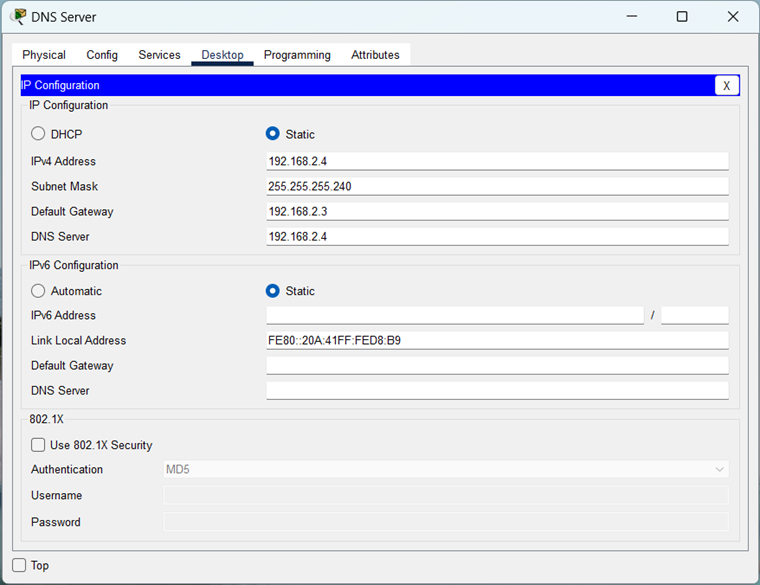
\includegraphics[width=1\textwidth]{dns_ip.png}
				\caption{Gán địa chỉ IP cho DNS Server thành công}
			\end{figure}
		\end{itemize}	
		\newpage
		\textbf{Bước 2: Tạo tên miền:} DNS Server → Services → DNS
		\begin{itemize}[leftmargin=0.75cm]
			\item DNS Service: On
			\item Name: saigonuniversity.com
			\item Address: 192.168.2.5 (IPv4 Address của Web Server)
			\item Chọn Add
			\begin{figure}[H]
				\centering
				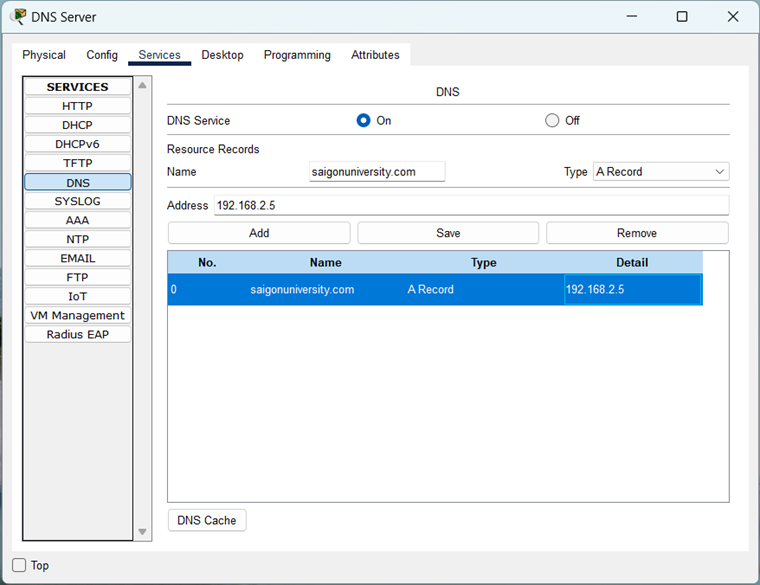
\includegraphics[width=1\textwidth]{dns_config.png}
				\caption{Cấu hình cho DNS Server}
			\end{figure}
		\end{itemize}
	\end{flushleft}

	\newpage
	\subsubsection{\textit{Web server và dịch vụ web}}
	\begin{flushleft}
		\textbf{Bước 1: Gán địa chỉ IP:} Web Server → Desktop → IP Configuration.
		\begin{itemize}[leftmargin=0.75cm]
			\item Chọn chế độ Static.
			\item IPv4 Address: 192.168.2.5
			\item Subnet Mask: 255.255.255.240
			\item Default Gateway: 192.168.2.3
			\item DNS server: 192.168.2.4
			\begin{figure}[H]
				\centering
				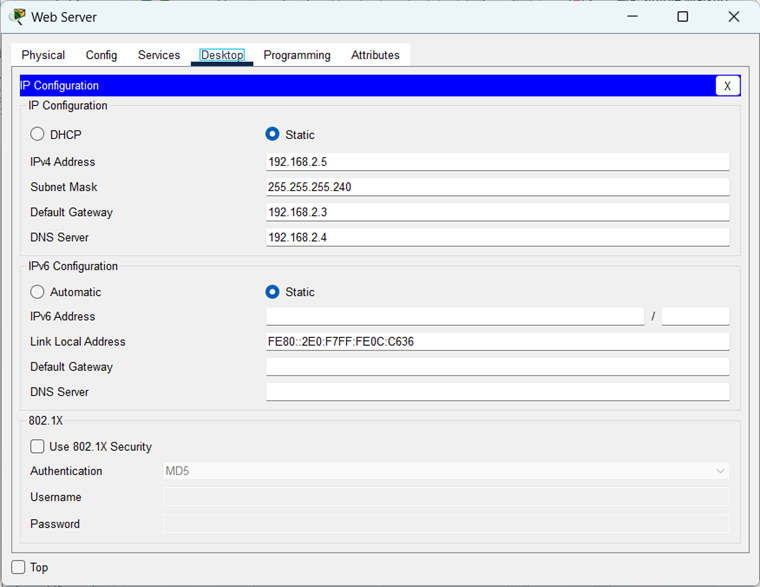
\includegraphics[width=1\textwidth]{web_ip.png}
				\caption{Gán địa chỉ IP cho Web Server thành công.}
			\end{figure}
		\end{itemize}
		\newpage
		\textbf{Bước 2: Tạo Web đơn giản bằng HTLM:}  Web Server → Services → HTTP
		\begin{itemize}[leftmargin=0.75cm]
			\item HTTP và HTTPS: On
			\item File Manager: Chưa các file .html và .jpg. Nếu muốn thêm file từ máy vào bấm chọn Import.
			\item Chỉnh sửa Web: chọn (edit) ở file index.html → Edit tùy ý → Save.
			\begin{figure}[H]
				\centering
				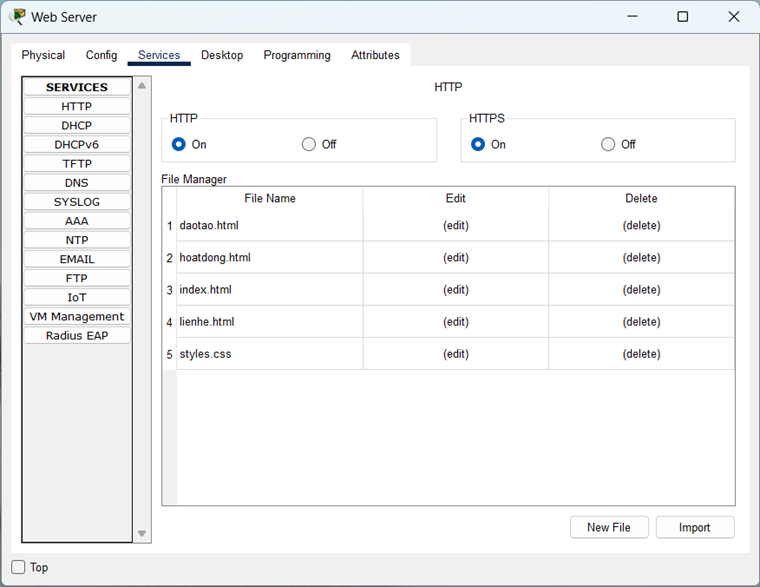
\includegraphics[width=1\textwidth]{web_accesshttp.png}
				\caption{Tạo web đơn giản}
			\end{figure}
		\end{itemize}
		\newpage
		\textbf{Bước 3: Truy cập Web:} Web Server → Desktop → Web Browser →  nhập địa chỉ vào URL → Go
		\begin{figure}[H]
			\centering
			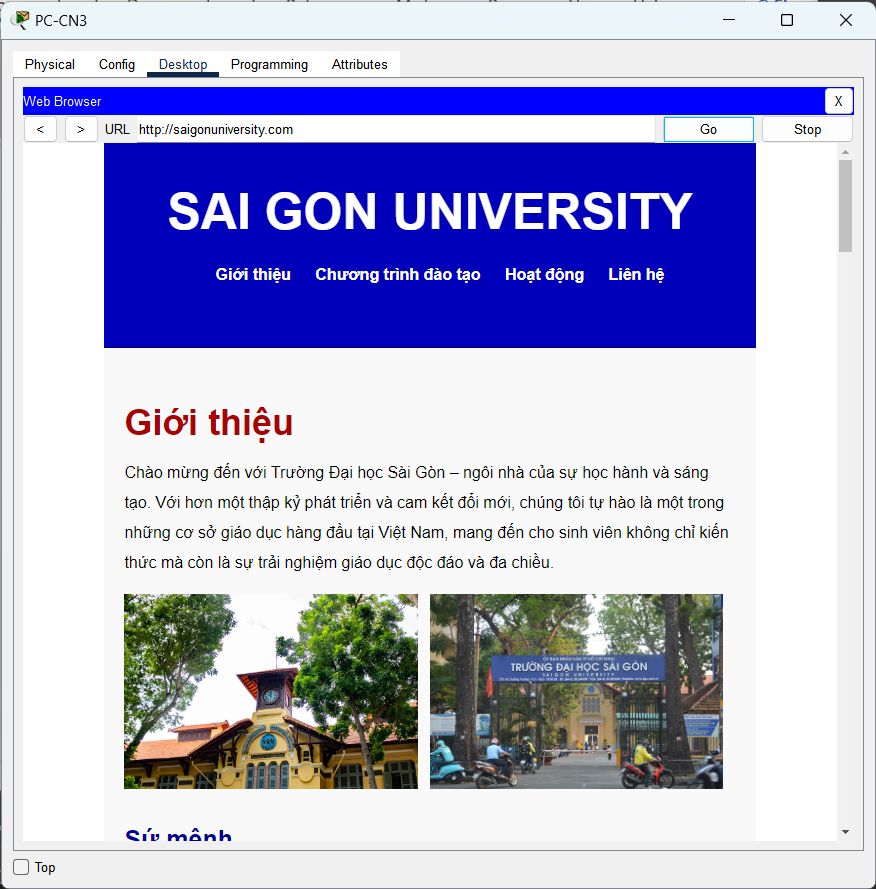
\includegraphics[width=1\textwidth]{web_creation.png}
			\caption{Truy cập Web thành công}
		\end{figure}
	\end{flushleft}
	
	\newpage
	\subsubsection{\textit{Mail server}}
	\begin{flushleft}
		\textbf{Bước 1: Gán địa chỉ IP:} Mail Server → Desktop → IP Configuration.
		\begin{itemize}[leftmargin=0.75cm]
			\item Chọn chế độ Static.
			\item IPv4 Address: 192.168.2.6
			\item Subnet Mask: 255.255.255.240
			\item Default Gateway: 192.168.2.3
			\item DNS server: 192.168.2.4
			\begin{figure}[H]
				\centering
				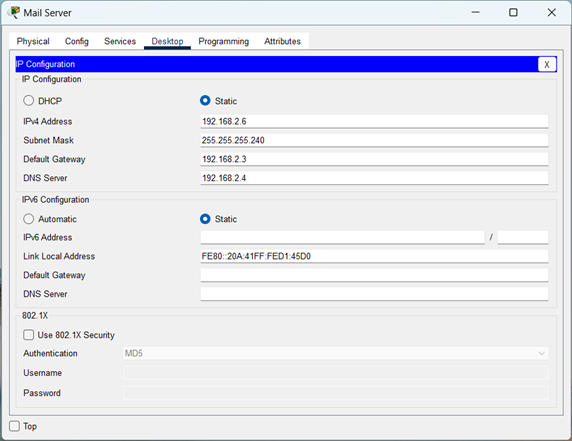
\includegraphics[width=1\textwidth]{mail_ip.png}
				\caption{Gán địa chỉ IP cho Mail Server thành công.}
			\end{figure}
		\end{itemize}
		\newpage
		\textbf{Bước 2: Tạo user:} Mail server → Services → EMAIL 
		\begin{itemize}[leftmargin=0.75cm]
			\item SMTP Service và POP3 Service: On
			\item Domain Name: gmail.com. 
			\item User: Tạo các tên tương ứng.
			\item Password: 123
			\item Chon “+”
			\begin{figure}[H]
				\centering
				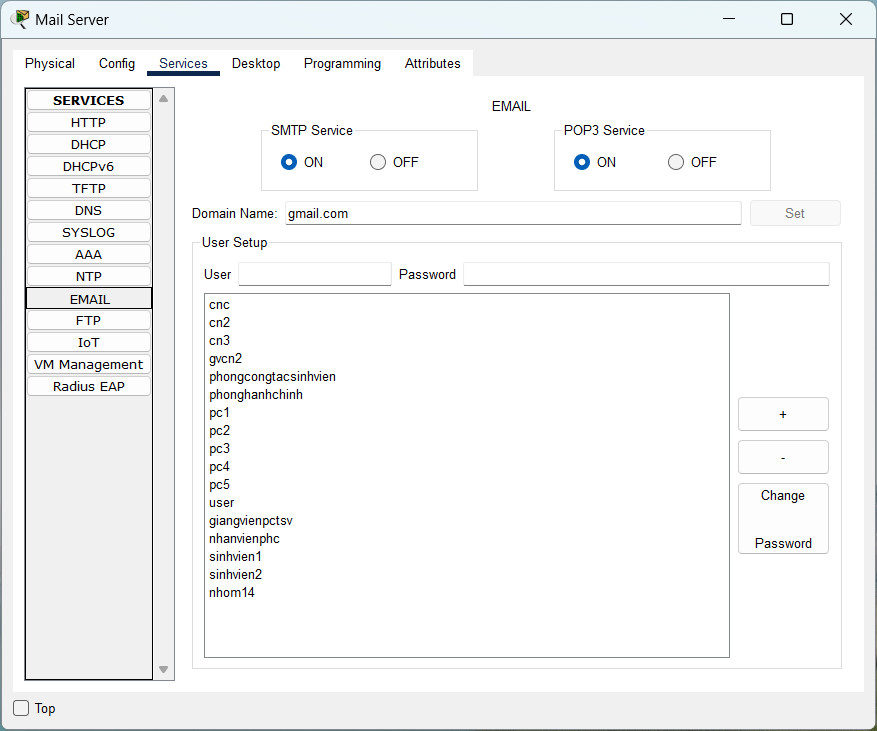
\includegraphics[width=1\textwidth]{users_creation.jpg}
				\caption{Tạo các tên người dùng}
			\end{figure}
		\end{itemize}
		\newpage
		\textbf{Bước 3: Cấu hình User Mail cho các thiết bị:} Desktop → Configure Mail 
		\begin{figure}[H]
			\centering
			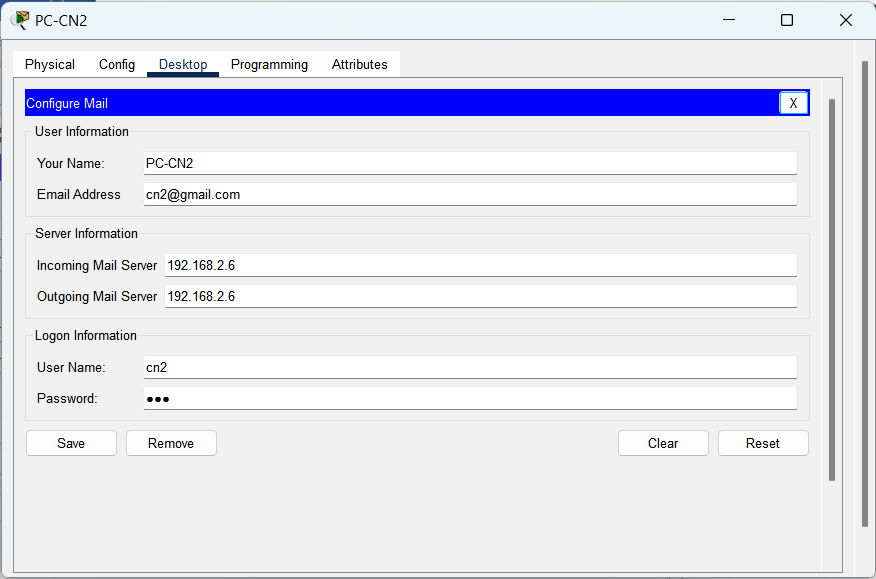
\includegraphics[width=1\textwidth]{users_config.png}
			\caption{Cấu hình User Mail cho các thiết bị}
		\end{figure}
		Các thiết bị khách làm tương tự, mật khẩu tất cả đều là 123.
		\begin{itemize}[leftmargin=0.75cm]
			\item PC-PĐT: cnc@gmail.com
			\item PC-PCTSV: phongctsv@gmail.com
			\item PC1 → PC5: pc1@gmail.com → pc5@gmail.com
			\item PC-CN2: cn2@gmail.com
			\item PC-CN3: cn3@gmail.com
			\item GV-CN2: gvcn2@gmail.com
			\item ...
		\end{itemize}
		\newpage
		\textbf{Bước 4: Test}
		\begin{itemize}[leftmargin=0.75cm]
			\item Chọn Compose để nhập nội dung gửi.
			\item Chọn Send để gửi.
			\item Chọn Receive từ thiết bị được nhận để nhận tin nhắn.
			\item Chọn Reply để trả lời tin nhắn. 
			\item Chọn Delete nếu muốn xóa nội dung tin nhắn đã gửi.
		\end{itemize}
		\textbf{Gửi mail từ các thiết bị}: Nhóm 15 chọn ra 3 PC ở cả 3 chi nhánh để tương tác với nhau. PC-CN2 sẽ gửi tin nhắn đến các PC-CN3 và PC-PĐT.
		\begin{figure}[H]
			\centering
			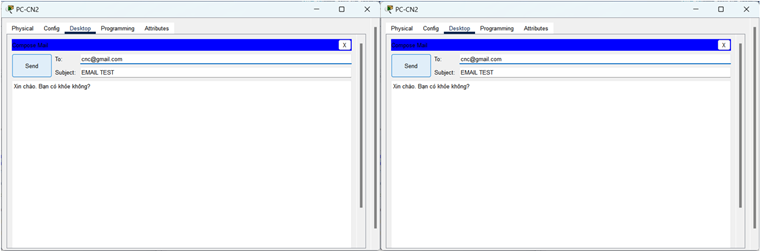
\includegraphics[width=1\textwidth]{devices_receivemail_01.png}
			\caption{PC-CN2 gửi tin nhắn đến các thiết bị}
		\end{figure}
		\begin{figure}[H]
			\centering
			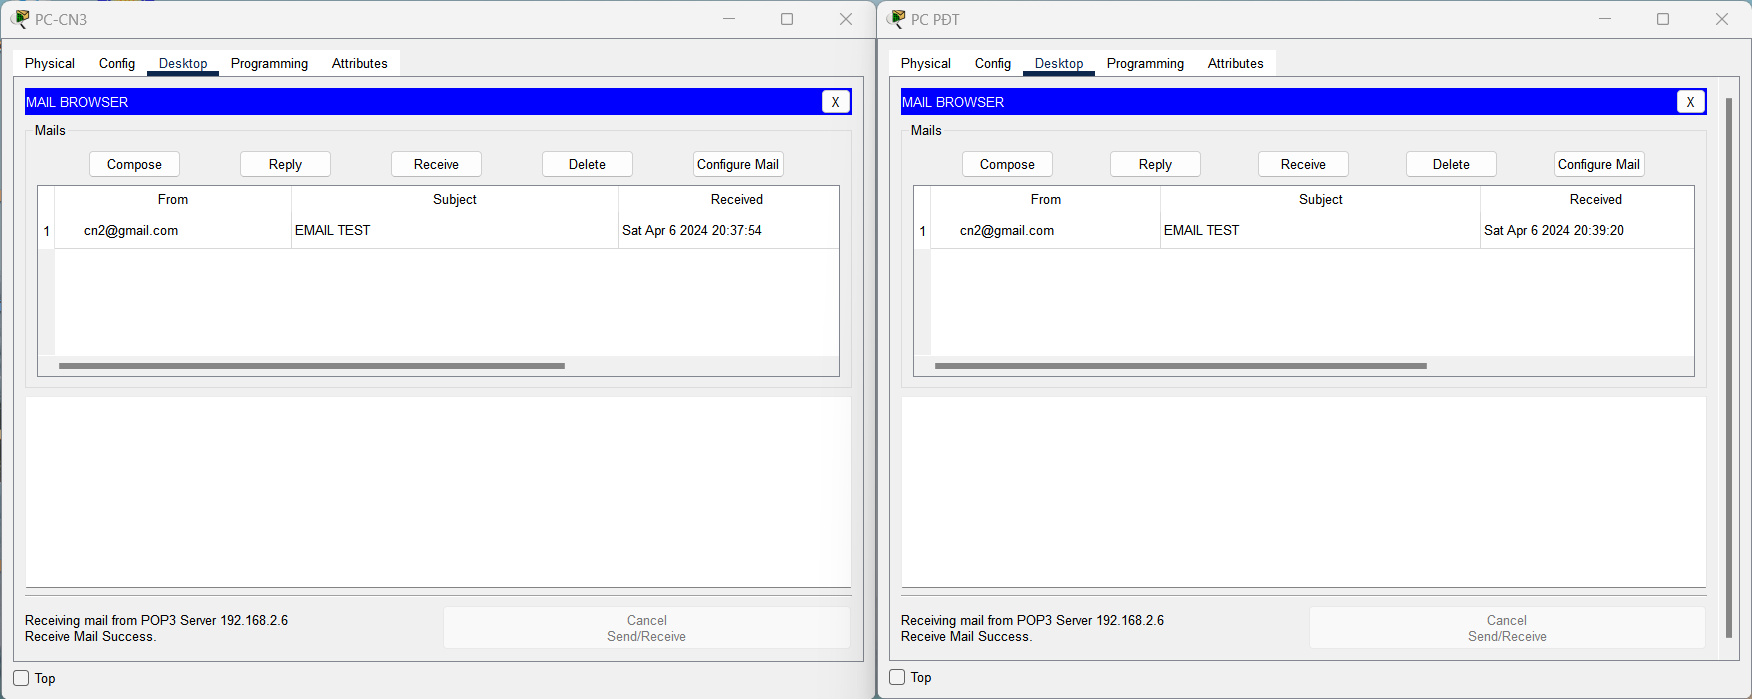
\includegraphics[width=1\textwidth]{devices_receivemail_03.png}
			\caption{PC-CN3 và PC-PĐT nhận email thành công}
		\end{figure}
		\newpage \textbf{Trả lời email}: Các PC đã nhận email từ PC-CN2 trả lời lại tin nhắn vừa nhận.
		\begin{figure}[H]
			\centering
			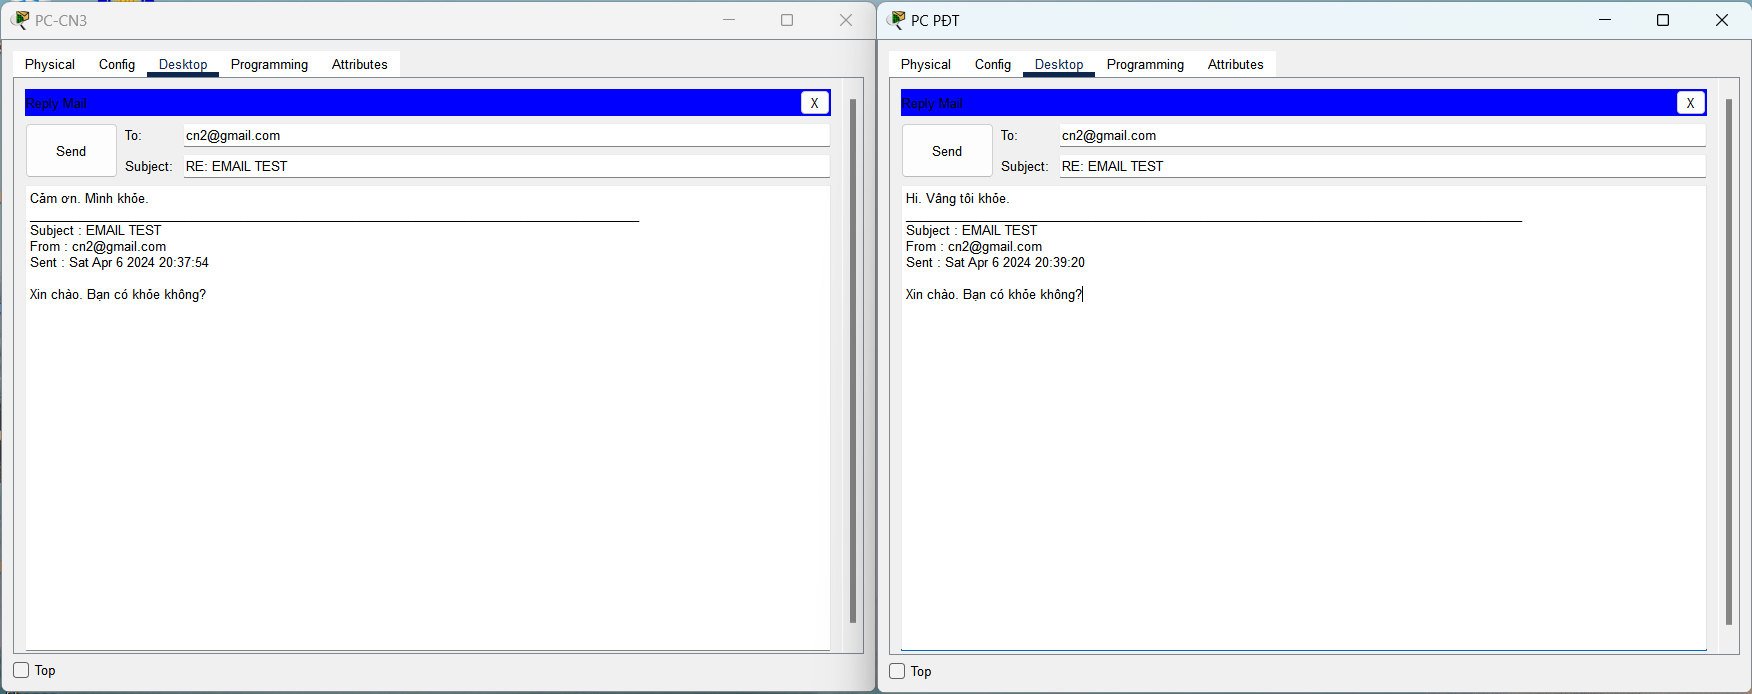
\includegraphics[width=1\textwidth]{reply_mail.png}
			\caption{PC-CN3 và PC-PĐT trả lời lại tin nhắn}
		\end{figure}
		\begin{figure}[H]
			\centering
			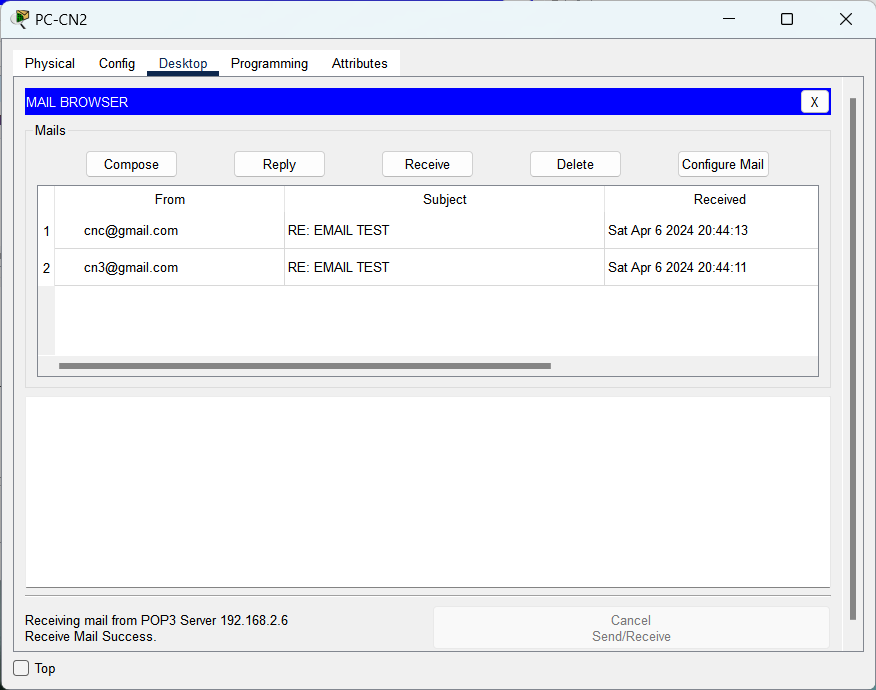
\includegraphics[width=1\textwidth]{sendandreply_steps.png}
			\caption{PC-CN2 nhận lại tin nhắn trả lời tahnfh công}
		\end{figure}
	\end{flushleft}
	
	\subsubsection{\textit{FTP Server}}
	\begin{flushleft}
		\textbf{Bước 1: Gán địa chỉ IP}: FTP Server → Desktop → IP Configuration.
		\begin{itemize}[leftmargin=0.75cm]
			\item Chọn chế độ Static.
			\item IPv4 Address: 192.168.2.7
			\item Subnet Mask: 255.255.255.240
			\item Default Gateway: 192.168.2.3
			\item DNS server: 192.168.2.4
			\begin{figure}[H]
				\centering
				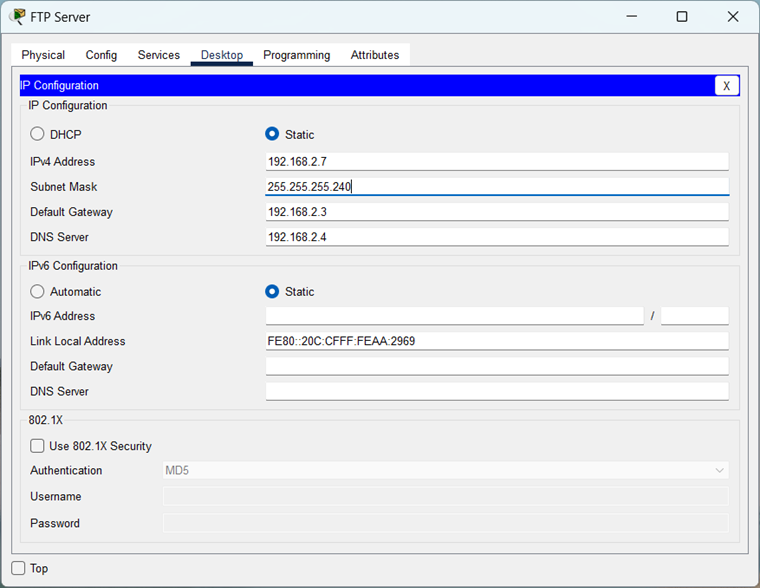
\includegraphics[width=1\textwidth]{ftp_ip.png}
				\caption{Gán địa chỉ IP cho FTP Server thành công.}
			\end{figure}
		\end{itemize}
		\newpage
		\textbf{Bước 2: Tạo tên người dùng:} FTP Server → Services → FTP
		\begin{itemize}[leftmargin=0.75cm]
			\item Service: On
			\item Username: Tên người dùng 
			\item Password: 123
			\item Bấm chọn tích các ô Write, Read, Delete, Rename, List. 
			\item Chọn Add.
			\begin{figure}[H]
				\centering
				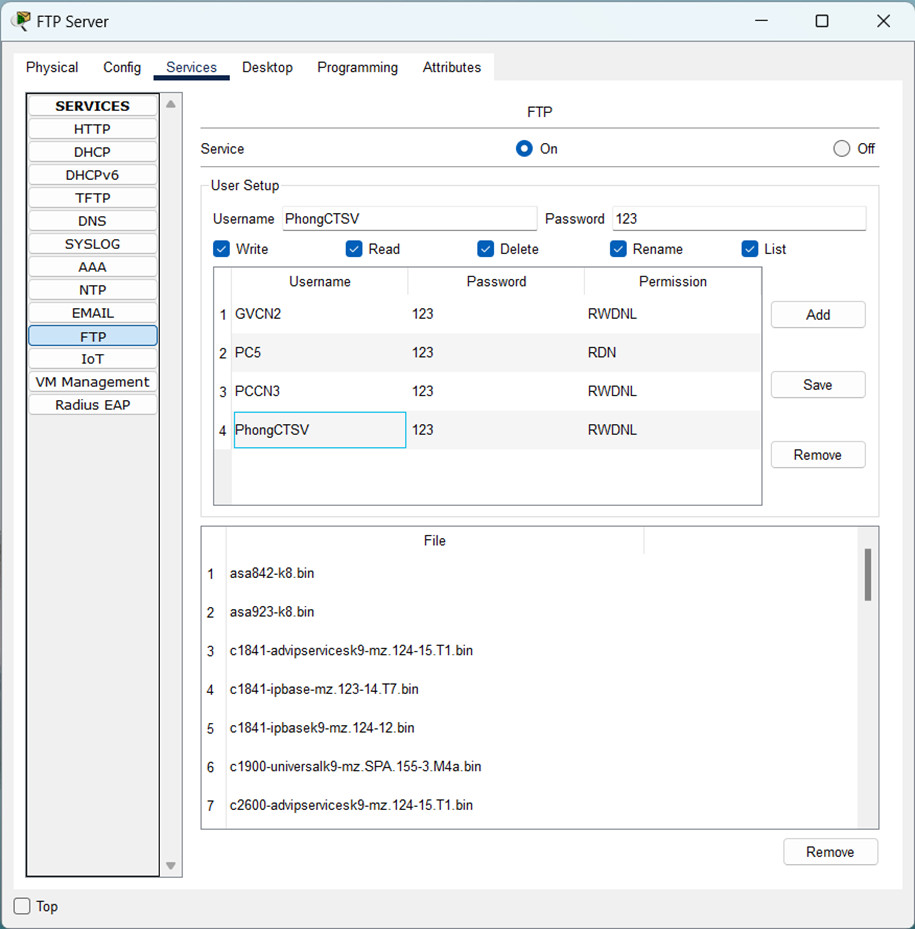
\includegraphics[width=0.95\textwidth]{ftp_config.jpg}
				\caption{Tạo tên người dùng}
			\end{figure}
		\end{itemize}
		\newpage
		\textbf{Bước 3: Kiểm tra}\\
		\begin{flushleft}
		Ở đây nhóm 15 chọn PC-CN3 ở CN3 để tạo, lưu file và dùng PC-PCTSV ở CNC để lấy dữ liệu.\\
		\end{flushleft}
		\textbf{Tạo và lưu file:} PC-CN3\\
		\begin{itemize}[leftmargin=0.75cm]
			\item Bước 1: Tạo một file hello.txt và bấm chọn File để lưu file.
			\begin{figure}[H]
				\centering
				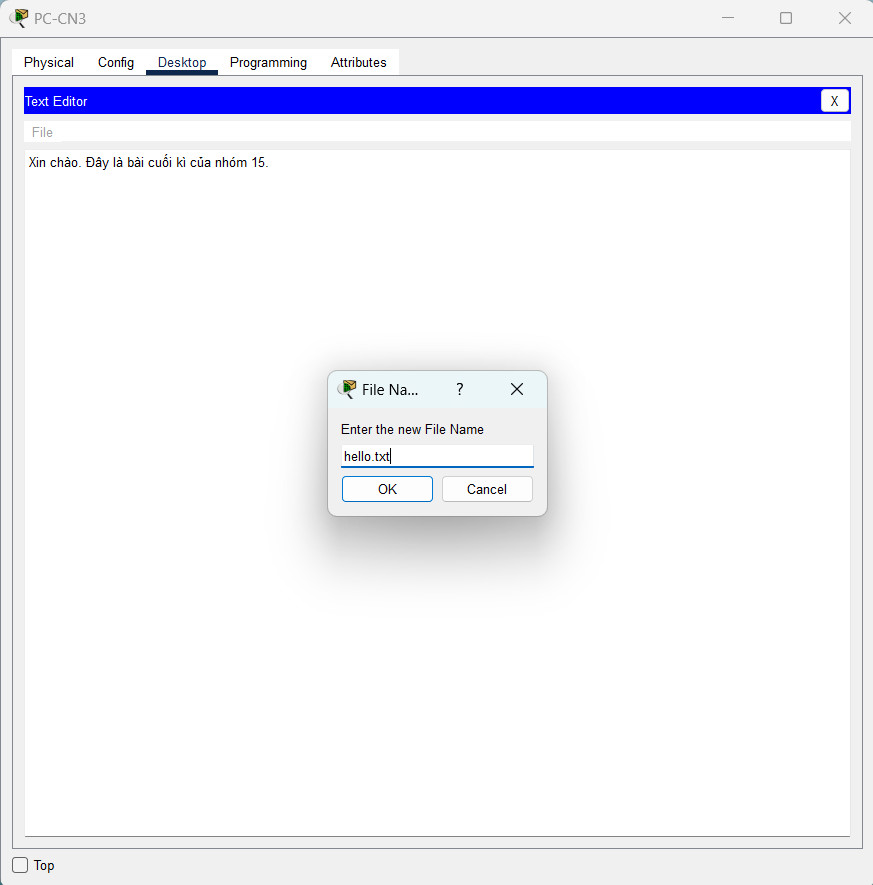
\includegraphics[width=1\textwidth]{hellofile_creation.jpg}
				\caption{Tạo file hello.txt}
			\end{figure}
			\newpage
			\item Bước 2: 
			\begin{itemize}[leftmargin=1cm] 
				\setstretch{1.5}
				\item Đẩy dữ liệu lên FTP server bằng cách đăng nhập Username và Password của FTP Server. 
				\item Sau đó, dùng lệnh ftp>put hello.txt
			\end{itemize}
			\begin{figure}[H]
				\centering
				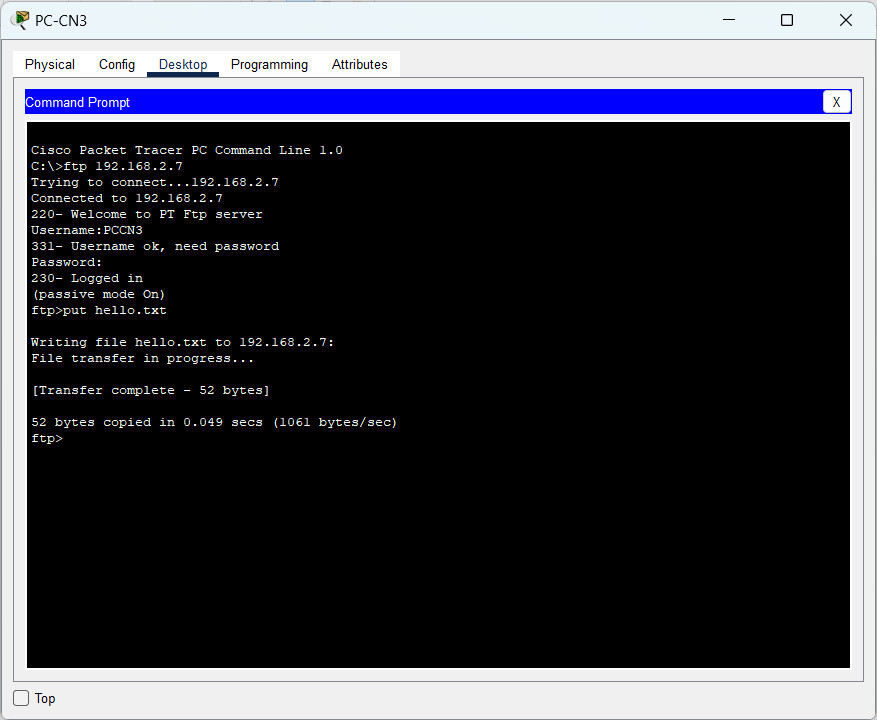
\includegraphics[width=1\textwidth]{ftp_dataupload.jpg}
				\caption{Đẩy dữ liệu lên FTP Server}
			\end{figure}
			\item Bước 3: Kiểm tra file đã được tải lên hay chưa bằng lệnh ftp>dir
			\begin{figure}[H]
				\centering
				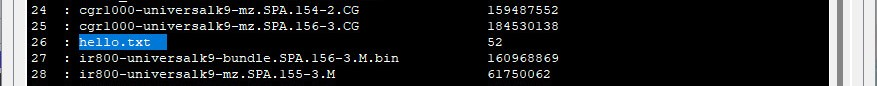
\includegraphics[width=1\textwidth]{data_uploadcompletely.jpg}
				\caption{Kiểm tra file đã được đẩy lên hay chưa}
			\end{figure}
		\end{itemize}
		\newpage
		\textbf{Tải file:} PC-PCTSV \\
		\begin{itemize}[leftmargin=0.75cm]
			\item Bước 1:
			\begin{itemize}[leftmargin=1cm] 
				\setstretch{1.5}
				\item Tải dữ liệu xuống từ FTP server bằng cách đăng nhập Username và Password của FTP Server. 
				\item Sau đó dùng lệnh ftp>get hello.txt để tải xuống file mà máy PC-PHC đã đẩy lên.
			\end{itemize}
			\begin{figure}[H]
				\centering
				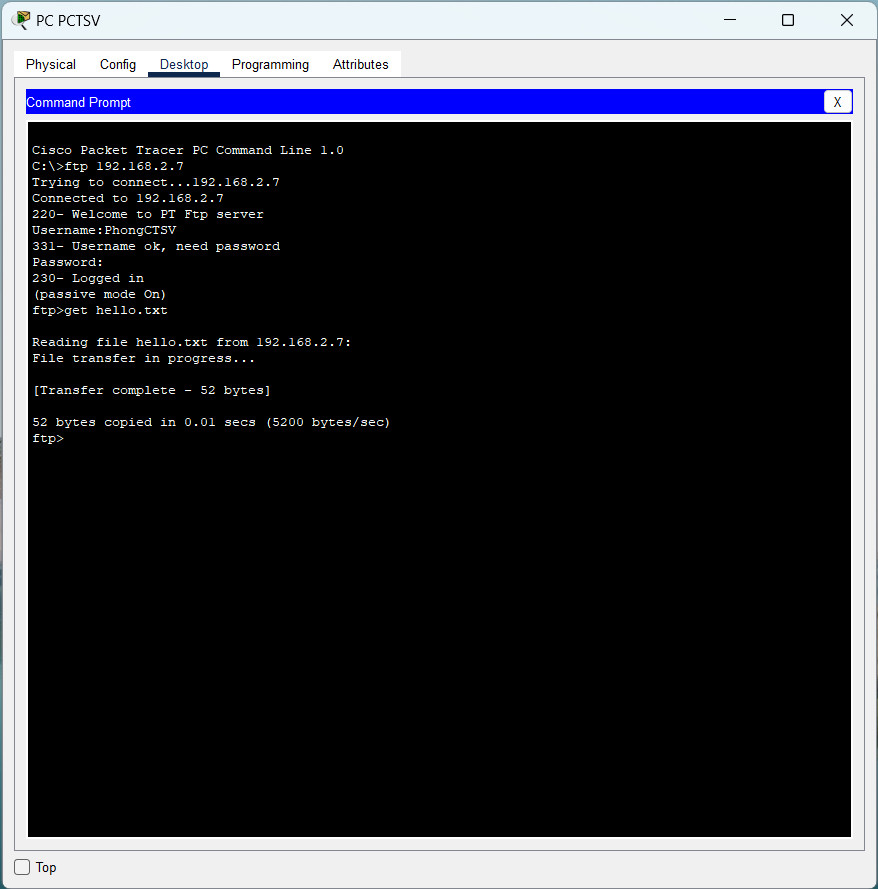
\includegraphics[width=1\textwidth]{ftp_datainstall.jpg}
				\caption{Tải dữ liệu xuống từ FTP Server}
			\end{figure}
			\newpage
			\item Bước 2: Kiểm tra file đã tải: Desktop → Text Editor → Ctrl + O
			\begin{figure}[H]
				\centering
				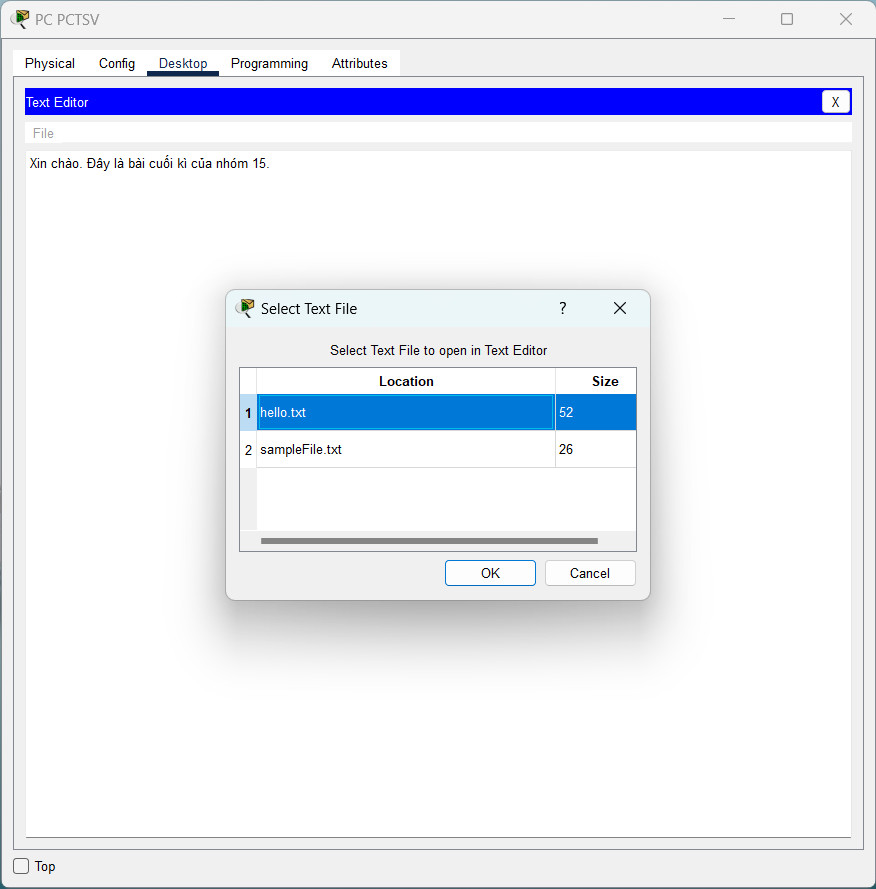
\includegraphics[width=1\textwidth]{data_installcompletely_01.jpg}
				\caption{Kiểm tra file đã tải}
			\end{figure}
			=> Đã tải được file hello.txt thành công.
		\end{itemize}
	\end{flushleft}
	\newpage
	\subsection{Cấu hình định tuyến OSPF}
	\begin{flushleft}
		\setstretch{1.5}
		\hspace{1.55cm}Cấu hình giao thức OSPF với các router R1, R2, R3, R4, RT-CN2, RT-CN3, RT-Active, RT-Backup, SW-CORE-1 và SW-CORE-2. Các câu lệnh cụ thể của từng thiết bị như sau:\\
	\end{flushleft}
	\begin{flushleft}
		+ Trên thiết bị R1:
		\begin{tcolorbox}
			router ospf 1\\
			network 1.1.1.0 0.0.0.255 area 0\\
			network 2.2.2.0 0.0.0.255 area 0\\
			network 8.8.8.8  0.0.0.255 area 0\\
			exit
		\end{tcolorbox}
		+ Trên thiết bị R2:
		\begin{tcolorbox}
			router ospf 1\\
			network 113.171.0.0 0.0.255.255 area 0\\
			network 2.2.2.0 0.0.0.255 area 0\\
			network 3.3.3.0 0.0.0.255 area 0\\
			exit
		\end{tcolorbox}
		+ Trên thiết bị R3: 
		\begin{tcolorbox}
			router ospf 1\\
			network 113.171.0.0 0.0.255.255 area 0\\
			network 3.3.3.0 0.0.0.255 area 0\\
			network 4.4.4.0 0.0.0.255 area 0\\
			exit
		\end{tcolorbox}
		\newpage
		+ Trên thiết bị R4: 
		\begin{tcolorbox}
			router ospf 1\\
			network 113.171.0.0 0.0.255.255 area 0\\
			network 1.1.1.0 0.0.0.255 area 0\\
			network 4.4.4.0 0.0.0.255 area 0\\
			exit
		\end{tcolorbox}
		+ Trên thiết bị RT-CN2: 
		\begin{tcolorbox}
			router ospf 1 \\
			network 113.171.0.0 0.0.255.255 area 0\\
			network 192.168.20.0 0.0.0.255 area 0\\
			exit
		\end{tcolorbox}
		+ Trên thiết bị RT-CN3: 
		\begin{tcolorbox}
			router ospf 1\\
			network 113.171.1.0 0.0.0.255 area 0\\
			network 192.168.30.0 0.0.0.255 area 0\\
			exit
		\end{tcolorbox}
		+ Trên thiết bị RT-Active: 
		\begin{tcolorbox}
			router ospf 1\\
			network 113.171.3.0 0.0.0.255 area 0\\
			network 10.0.2.0 0.0.0.255 area 0 \\
			default-information originate
		\end{tcolorbox}
		\newpage
		+ Trên thiết bị RT-Backup: 
		\begin{tcolorbox}
			\setstretch{1.45}
			router ospf 1\\
			network 113.171.2.0 0.0.0.255 area 0\\
			network 10.0.3.0 0.0.0.255 area 0\\
			default-information originate
		\end{tcolorbox}
		+ Trên thiết bị SW-CORE-1: 
		\begin{tcolorbox}
			\setstretch{1.45}
			router ospf 1\\
			network 10.0.1.0 0.0.0.255 area 0\\
			network 10.0.2.0 0.0.0.255 area 0\\
			network 192.168.0.0 0.0.0.255 area 0\\
			network 192.168.1.0 0.0.0.127 area 0\\
			network 192.168.1.128 0.0.0.63 area 0\\
			network 192.168.1.192 0.0.0.63 area 0\\
			network 192.168.2.0 0.0.0.7 area 0
		\end{tcolorbox}
		+ Trên thiết bị SW-CORE-2: 
		\begin{tcolorbox}
			\setstretch{1.45}
			router ospf 1\\
			network 10.0.1.0 0.0.0.255 area 0\\
			network 10.0.3.0 0.0.0.255 area 0\\
			network 192.168.0.0 0.0.0.255 area 0\\
			network 192.168.1.0 0.0.0.127 area 0\\
			network 192.168.1.128 0.0.0.63 area 0\\
			network 192.168.1.192 0.0.0.63 area 0\\
			network 192.168.2.0 0.0.0.7 area 0
		\end{tcolorbox}
	\end{flushleft}
	
	\newpage
	\subsection{Cấu hình STP và HSRP}
	\subsubsection{\textit{Cấu hình STP}}
	\begin{flushleft}
		- Trên thiết bị SW-CORE-1, ưu tiên đường đi của VLAN 10, VLAN11, VLAN 12. Cấu hình như sau:
		\begin{tcolorbox}
			spanning-tree mode rapid\\
			spanning-tree vlan 10 root primary\\
			spanning-tree vlan 11 root primary\\
			spanning-tree vlan 12 root primary\\
			spanning-tree vlan 13 root secondary\\
			spanning-tree vlan 14 root secondary\\
			end
		\end{tcolorbox}
		- Và trên thiết bị SW-CORE-2, ưu tiên đường đi của các VLAN còn lại. Cấu hình như sau:
		\begin{tcolorbox}
			spanning-tree mode rapid\\
			spanning-tree vlan 10 root secondary\\
			spanning-tree vlan 11 root secondary\\
			spanning-tree vlan 12 root secondary\\ 
			spanning-tree vlan 13 root primary\\ 
			spanning-tree vlan 14 root primary\\
			end
		\end{tcolorbox}
		- Để kiểm tra các thiết bị đã cấu hình thành công hay chưa, trên các SW-CORE gõ lệnh: spanning-tree mode rapid
	\end{flushleft}
	\newpage
	\subsubsection{\textit{Cấu hình HSRP}}
	\begin{flushleft}
		- Trên thiết bị SW-CORE-1, ưu tiên đường đi của VLAN 10, VLAN11, VLAN 12. Cấu hình như sau:
		\begin{tcolorbox}
			\setstretch{1.2}
			config t \\
			int vlan 10\\
			standby 1 ip 192.168.2.3\\
			standby 1 priority 105\\
			standby 1 preempt\\
			exit\\
			int vlan 11\\
			standby 1 ip 192.168.1.195\\
			standby 1 priority 105\\
			standby 1 preempt\\
			exit\\
			int vlan 12\\
			standby 1 ip 192.168.1.131\\
			standby 1 priority 105\\
			standby 1 preempt\\
			exit\\
			int vlan 13\\
			standby 1 ip 192.169.1.3\\
			standby 1 priority 95\\
			standby 1 preempt\\
			exit\\
			int vlan 14 \\
			standby 1 ip 192.168.0.3\\
			standby 1 priority 95\\
			standby 1 preempt\\
			exit
		\end{tcolorbox}
		- Và trên thiết bị SW-CORE-2, ưu tiên đường đi của các VLAN còn lại. Cấu hình như sau:
		\begin{tcolorbox}
			\setstretch{1.3}
			config t\\
			int vlan 10\\
			standby 1 ip 192.168.2.3\\
			standby 1 priority 95\\
			standby 1 preempt\\
			exit\\
			int vlan 11\\
			standby 1 ip 192.168.1.195\\
			standby 1 priority 95\\
			standby 1 preempt\\
			exit\\
			int vlan 12\\
			standby 1 ip 192.168.1.131\\
			standby 1 priority 95\\
			standby 1 preempt\\
			exit\\
			int vlan 13\\
			standby 1 ip 192.168.1.3\\
			standby 1 priority 105\\
			standby 1 preempt\\
			exit\\
			int vlan 14\\
			standby 1 ip 192.168.0.3\\
			standby 1 priority 105\\
			standby 1 preempt\\
			exit
		\end{tcolorbox}
	\end{flushleft}
	\subsection{Cấu hình Wifi}
	\begin{flushleft}
		\textbf{Bước 1: Cài đặt địa chỉ IP} \\
		\hspace{1cm}Chọn thiết bị → GUI → Ở phần Internet Setup chọn IP DHCP để nhận IP động theo từng đường mạng.\\
		\textbf{Bước 2: Cấu hình Wireless}\\
		 \hspace{1cm}Chuyển sang tab Wireless → Nhập các thông tin dưới đây đối với mạng 2.4GHz, cũng như cho hai kênh 5GHz-1 và 5GHz-2.
		\begin{itemize}[leftmargin=1.75cm, itemsep=0pt, topsep=0pt]
			\item Network Mode: Auto
			\item Network name (SSID): <Đặt tùy chọn>
			\item Standard Channel: Auto
			\item Channel Bandwidth: Auto
		\end{itemize}
		\hspace{1cm}Sau khi nhập thông tin → Nhấn Save Settings ở cuối trang.\\
		\textbf{Bước 3: Đặt mật khẩu cho Wireless}\\
		\hspace{1cm}Chọn tab Wireless → Chọn Wireless Security C → Nhập thông tin dưới đây cho 2.4GHz, đồng thời làm tương tự cho 2 kênh 5GHz-1 và 5GHz-2. 
		\begin{itemize}[leftmargin=1.75cm, itemsep=0pt, topsep=0pt]
			\item Security Mode: WPA Personal
			\item Encryption: AES
			\item Passphrase: saigonuniversity
		\end{itemize}
		\hspace{1cm}Sau khi nhập thông tin → Nhấn Save Settings ở cuối trang.\\
		\newpage
		\textbf{Bước 4: Áp dụng vào các WiFi hiện có trong bài}
		\\- Chọn WiFi PĐT để cấu hình, các WiFi còn lại làm tương tự.
		\\- Đầu tiên, vào xem địa chỉ Internet được cấp động xuống.
		\begin{figure}[H]
			\centering
			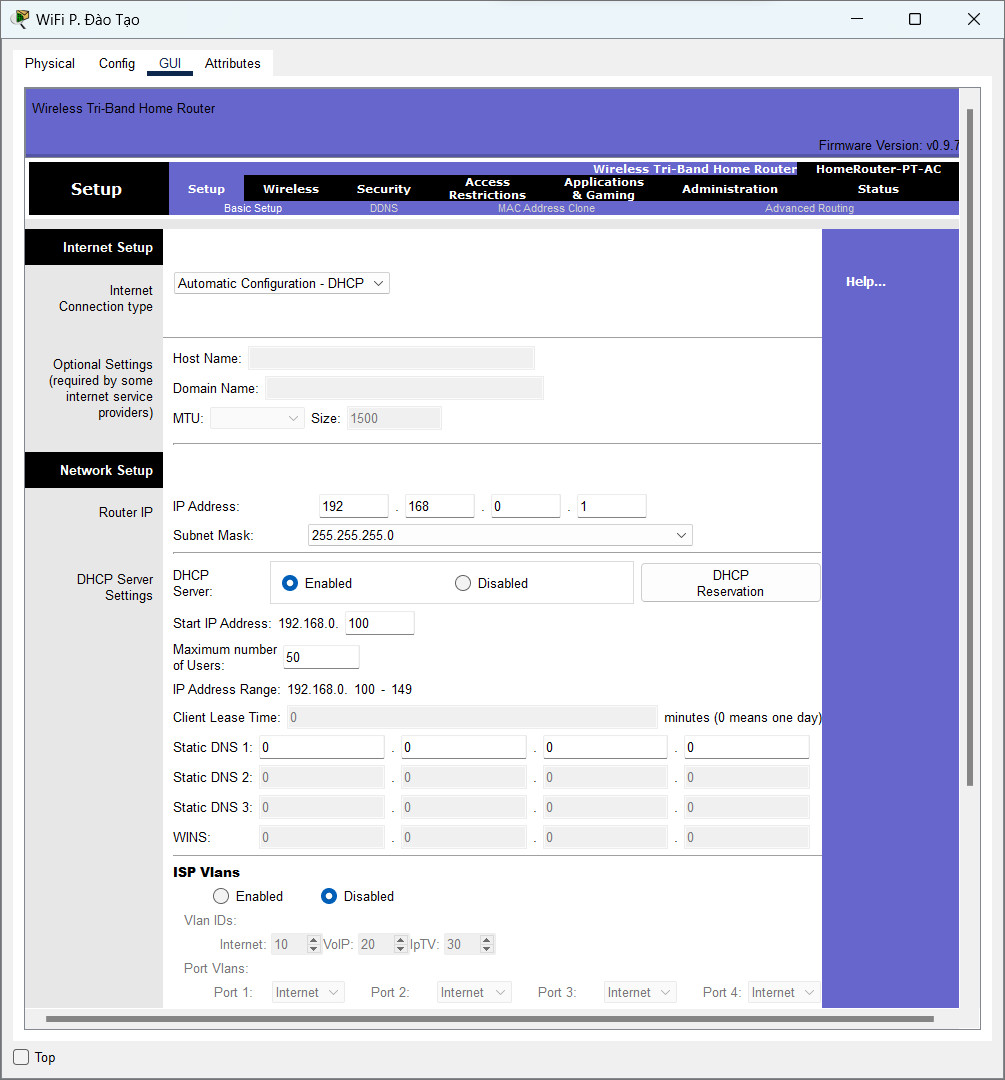
\includegraphics[width=1\textwidth]{wifi_internet.jpg}
			\caption{Cài đặt địa chỉ Internet}
		\end{figure}
		\newpage
		- Sau đó, cấu hình wireless.
		\begin{figure}[H]
			\centering
			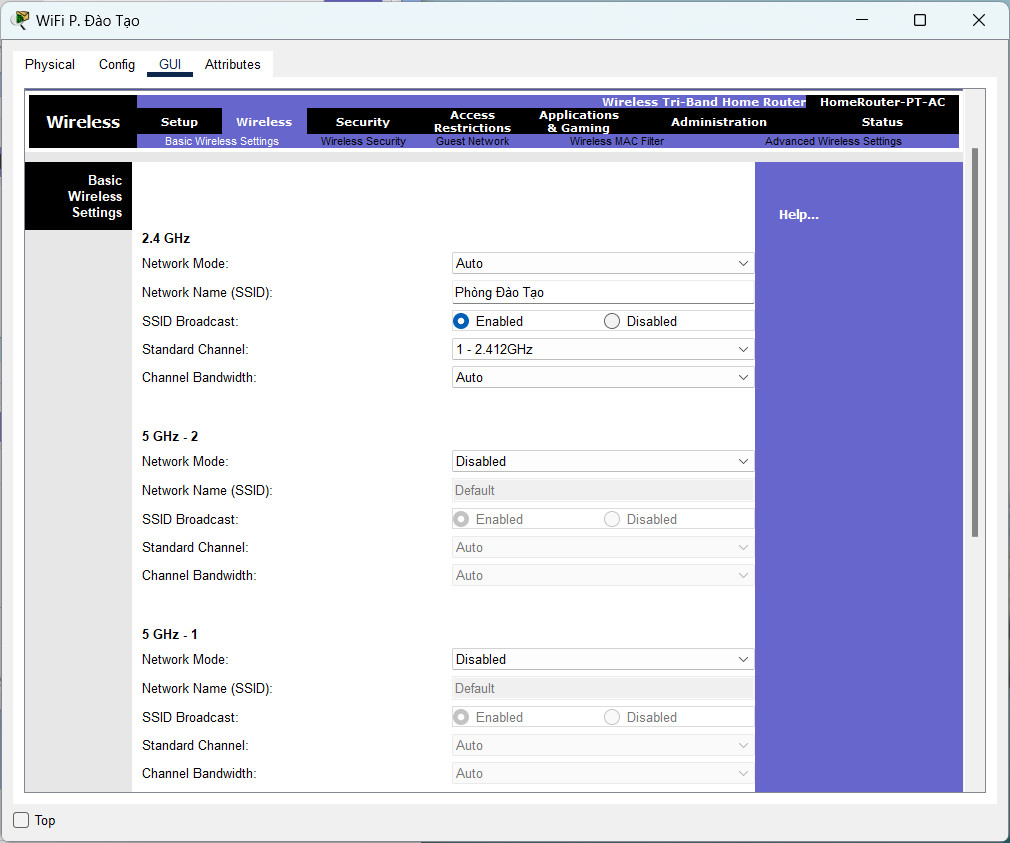
\includegraphics[width=1\textwidth]{wifi_wlc.jpg}            	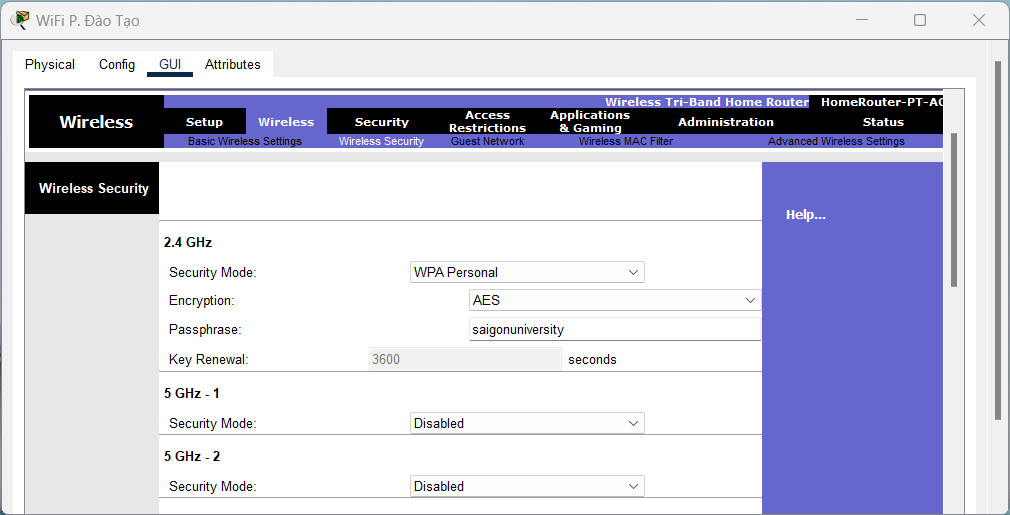
\includegraphics[width=1\textwidth]{wifi_wlc_security.jpg}
			\caption{Cài đặt wireless}
		\end{figure}
		\newpage
		- Vào 1 thiết bị khác để kiểm tra thử. Chọn Smarphone-ToaA để kiểm tra.
		\begin{figure}[H]
			\centering
			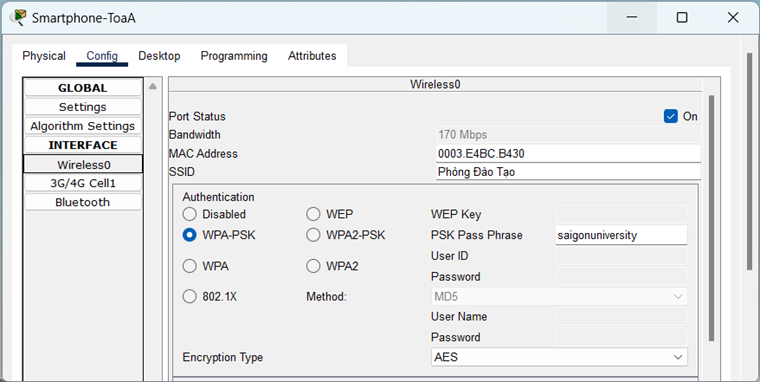
\includegraphics[width=1\textwidth]{test-wifi-1.png}
			\caption{Thiết bị kết nối vào wifi}  
			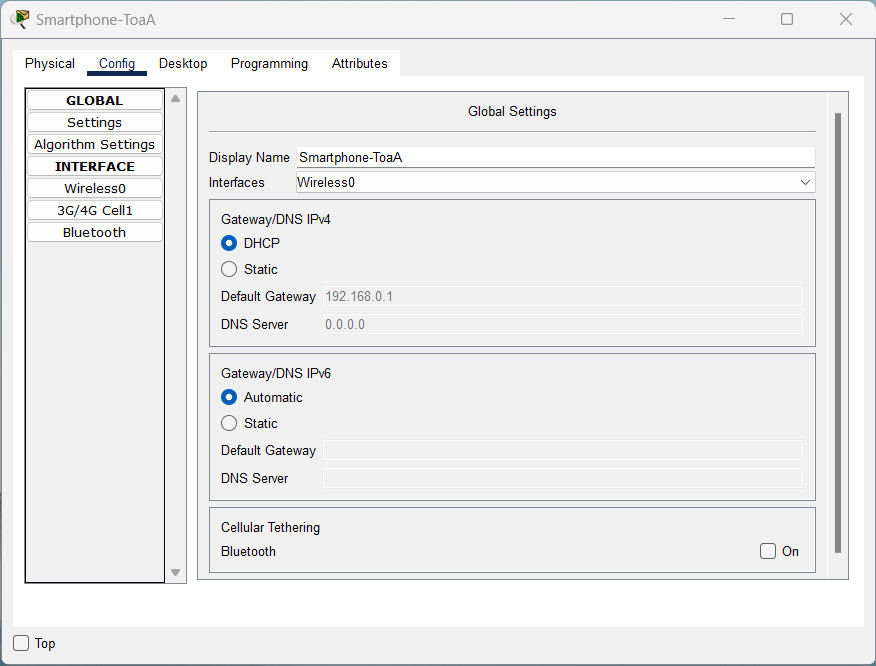
\includegraphics[width=1\textwidth]{test-wifi-2.jpg}
			\caption{Thiết bị nhận địa chỉ IP thành công}
		\end{figure}
	\end{flushleft}
	\newpage
	\section{KẾT LUẬN VÀ HƯỚNG PHÁT TRIỂN}
	\subsection{Kết quả đạt được}
	\hspace{1.5cm}Sau khi hoàn thiện xong đồ án này, tổng thể mạng của nhóm 15 đã được thiết kế, cấu hình hoàn chỉnh và gán đầy đủ các địa chỉ IP trên phần mềm Cisco Packet.
	\par
	\hspace{0.9cm}Các thiết bị sau khi cấu hình đã hoạt động và đáp ứng được một số yêu cầu như cấu hình DHCP cho các thiết bị nhận địa chỉ IP, cấu hình OSPF, cấu hình một số loại server như: DNS, DHCP, Web, Mail, FTP và chia VLAN, định tuyến VLAN.
	
	\subsection{Hạn chế}
	\hspace{1.5cm}Mặc dù dự án đã đạt được nhiều kết quả tích cực, vẫn còn một số hạn chế cần khắc phục. Cụ thể, việc quản lý và bảo mật mạng vẫn chưa được tối ưu hoàn toàn, và một số tính năng nâng cao chưa được triển khai đầy đủ do hạn chế về thời gian và tài nguyên.
	
	\subsection{Định hướng}
	\hspace{1.5cm}Trong tương lai, nhóm dự án sẽ tiếp tục cải tiến và hoàn thiện hệ thống mạng. Các bước tiếp theo bao gồm tối ưu hóa bảo mật, triển khai thêm các tính năng nâng cao và thực hiện các thử nghiệm để đảm bảo tính ổn định và hiệu quả của hệ thống. Đồng thời, nhóm cũng sẽ tìm hiểu và áp dụng các công nghệ mạng mới nhằm nâng cao hiệu suất và tính bảo mật của hệ thống.
	
	\newpage
	\section{TÀI LIỆU THAM KHẢO}
	\setlength{\parindent}{1.5cm}
	\textbf{Tiếng Việt}\\
	\large 1. Nguyễn Thúc Hải (1997), \textit{Mạng máy tính và các hệ thống mở}, NXB Giáo dục.\\
	\large 2. Phạm Thế Quế (2008), \textit{Công nghệ Mạng máy tính}, NXB Bưu điện.\\
	\large 3. Ngô Bá Hùng (2005), \textit{Giáo trình Thiết kế - Cài đặt mạng}, Đại học Cần Thơ.\\
	\textbf{Tiếng Anh}\\
	\large 4. Mimi Dutta (2023), \textit{CCNA Introducing Network Design Concepts}, Analytics Vidhya.\\
	\large 5. Bishop, Christopher M. (2006), \textit{Pattern Recognition and Machine Learning}, Springer.
\end{document}

